%%%%%%%%%%%%%%%%%%%%%%%%%%%%%%%%%%%%%%%%%
% Masters/Doctoral Thesis 
% LaTeX Template
% Version 2.5 (27/8/17)
%
% This template was downloaded from:
% http://www.LaTeXTemplates.com
%
% Version 2.x major modifications by:
% Vel (vel@latextemplates.com)
%
% This template is based on a template by:
% Steve Gunn (http://users.ecs.soton.ac.uk/srg/softwaretools/document/templates/)
% Sunil Patel (http://www.sunilpatel.co.uk/thesis-template/)
%
% Template license:
% CC BY-NC-SA 3.0 (http://creativecommons.org/licenses/by-nc-sa/3.0/)
%
%%%%%%%%%%%%%%%%%%%%%%%%%%%%%%%%%%%%%%%%%

%----------------------------------------------------------------------------------------
%	PACKAGES AND OTHER DOCUMENT CONFIGURATIONS
%----------------------------------------------------------------------------------------

\documentclass[
11pt, % The default document font size, options: 10pt, 11pt, 12pt
%oneside, % Two side (alternating margins) for binding by default, uncomment to switch to one side
english, % ngerman for German
singlespacing, % Single line spacing, alternatives: onehalfspacing or doublespacing
%draft, % Uncomment to enable draft mode (no pictures, no links, overfull hboxes indicated)
%nolistspacing, % If the document is onehalfspacing or doublespacing, uncomment this to set spacing in lists to single
%liststotoc, % Uncomment to add the list of figures/tables/etc to the table of contents
%toctotoc, % Uncomment to add the main table of contents to the table of contents
%parskip, % Uncomment to add space between paragraphs
%nohyperref, % Uncomment to not load the hyperref package
headsepline, % Uncomment to get a line under the header
%chapterinoneline, % Uncomment to place the chapter title next to the number on one line
%consistentlayout, % Uncomment to change the layout of the declaration, abstract and acknowledgements pages to match the default layout
]{MastersDoctoralThesis} % The class file specifying the document structure

\usepackage[utf8]{inputenc} % Required for inputting international characters
\usepackage[T1]{fontenc} % Output font encoding for international characters

\usepackage{mathpazo} % Use the Palatino font by default

\usepackage[backend=bibtex,style=authoryear,natbib=true]{biblatex} % Use the bibtex backend with the authoryear citation style (which resembles APA)

\addbibresource{example.bib} % The filename of the bibliography

\usepackage[autostyle=true]{csquotes} % Required to generate language-dependent quotes in the bibliography

\usepackage[colorlinks=true,linkcolor=blue]{hyperref}
\usepackage{graphicx}
\usepackage{float}


\def\cmay   {{\bf CMAY}}
\def\cmen   {{\bf CMEN}}
\def\aum    {{\bf AUM }}
\def\agnoff  {{\bf AGN-OFF }}
\def\hr  {{\bf HR }}
\def\mr  {{\bf MR }}


%----------------------------------------------------------------------------------------
%	MARGIN SETTINGS
%----------------------------------------------------------------------------------------

\geometry{
	paper=a4paper, % Change to letterpaper for US letter
	inner=2.5cm, % Inner margin 2.5
	outer=2.5cm, % Outer margin 3.8
	bindingoffset=.5cm, % Binding offset
	top=1.5cm, % Top margin
	bottom=1.5cm, % Bottom margin
	%showframe, % Uncomment to show how the type block is set on the page
}

%----------------------------------------------------------------------------------------
%	THESIS INFORMATION
%----------------------------------------------------------------------------------------

\thesistitle{Galaxias Centrales de C\'umulos Masivos en Simulaciones Cosmol\'ogicas Hidrodin\'amicas} % Your thesis title, this is used in the title and abstract, print it elsewhere with \ttitle
\supervisor{Dra. Cinthia Ragone-Figueroa} % Your supervisor's name, this is used in the title page, print it elsewhere with \supname
\examiner{} % Your examiner's name, this is not currently used anywhere in the template, print it elsewhere with \examname
\degree{Licenciada en Astronom\'ia} % Your degree name, this is used in the title page and abstract, print it elsewhere with \degreename
\author{Mar\'ia Eugenia Ferraro} % Your name, this is used in the title page and abstract, print it elsewhere with \authorname
\addresses{} % Your address, this is not currently used anywhere in the template, print it elsewhere with \addressname

\subject{Astronom\'ia Extragal\'actica} % Your subject area, this is not currently used anywhere in the template, print it elsewhere with \subjectname
\keywords{} % Keywords for your thesis, this is not currently used anywhere in the template, print it elsewhere with \keywordnames
\university{\href{http://www.university.com}{Universidad Nacional de C\'ordoba}} % Your university's name and URL, this is used in the title page and abstract, print it elsewhere with \univname
\department{\href{http://department.university.com}{Facultad de Matem\'atica, Astrnom\'ia, F\'isica y Computaci\'on}} % Your department's name and URL, this is used in the title page and abstract, print it elsewhere with \deptname
\group{\href{http://researchgroup.university.com}} % Your research group's name and URL, this is used in the title page, print it elsewhere with \groupname
\faculty{\href{http://faculty.university.com}{Facultad de Matem\'atica, Astrnom\'ia, F\'isica y Computaci\'on}} % Your faculty's name and URL, this is used in the title page and abstract, print it elsewhere with \facname

\AtBeginDocument{
\hypersetup{pdftitle=\ttitle} % Set the PDF's title to your title
\hypersetup{pdfauthor=\authorname} % Set the PDF's author to your name
\hypersetup{pdfkeywords=\keywordnames} % Set the PDF's keywords to your keywords
}

\begin{document}

\frontmatter % Use roman page numbering style (i, ii, iii, iv...) for the pre-content pages

\pagestyle{plain} % Default to the plain heading style until the thesis style is called for the body content

%----------------------------------------------------------------------------------------
%	TITLE PAGE
%----------------------------------------------------------------------------------------

\begin{titlepage}
\begin{center}

\vspace*{-1cm}
{\scshape\LARGE \univname\par}\vspace{1cm} % University name

\includegraphics[width=6cm]{Figures/uni.jpg} \\ \medskip % Picture
\textsc{\Large Tesis de Licenciatura}\\[0.5cm] % Thesis type


\HRule \\[0.4cm] % Horizontal line
{\huge \bfseries \ttitle\par}\vspace{0.4cm} % Thesis title
\HRule \\[1.5cm] % Horizontal line
 
\begin{minipage}[t]{0.4\textwidth}
\begin{flushleft} \large
\emph{Autor:}\\
\href{http://www.johnsmith.com}{\authorname} % Author name - remove the \href bracket to remove the link
\end{flushleft}
\end{minipage}
\begin{minipage}[t]{0.4\textwidth}
\begin{flushright} \large
\emph{Director:} \\
\href{http://www.jamessmith.com}{\supname} % Supervisor name - remove the \href bracket to remove the link  
\end{flushright}
\end{minipage}\\[3cm]
 
\large \textit{Tesis presentada en cumplimiento de los requisitos\\ para el grado de \degreename}\\[0.3cm] % University requirement text
\textit{en la}\\[0.4cm]
\deptname\\[2cm] % Research group name and department name
 
\vspace*{-1cm}
{\large \today}\\[4cm] % Date
%\includegraphics{Logo} % University/department logo - uncomment to place it
 
\vfill
\end{center}
\end{titlepage}

%----------------------------------------------------------------------------------------
%	DECLARATION PAGE
%----------------------------------------------------------------------------------------

\begin{declaration}
%\addchaptertocentry{\authorshipname} % Add the declaration to the table of contents
%\noindent I, \authorname, declare that this thesis titled, \enquote{\ttitle} and the work presented in it are my own. I confirm that:

%\begin{itemize} 
%\item This work was done wholly or mainly while in candidature for a research degree at this University.
%\item Where any part of this thesis has previously been submitted for a degree or any other qualification at this University or any other institution, this has been clearly stated.
%\item Where I have consulted the published work of others, this is always clearly attributed.
%\item Where I have quoted from the work of others, the source is always given. With the exception of such quotations, this thesis is entirely my own work.
%\item I have acknowledged all main sources of help.
%\item Where the thesis is based on work done by myself jointly with others, I have made clear exactly what was done by others and what I have contributed myself.\\
%\end{itemize}
 
%\noindent Signed:\\
%\rule[0.5em]{25em}{0.5pt} % This prints a line for the signature
 
%\noindent Date:\\
%\rule[0.5em]{25em}{0.5pt} % This prints a line to write the date
\end{declaration}

\cleardoublepage

%----------------------------------------------------------------------------------------
%	QUOTATION PAGE
%----------------------------------------------------------------------------------------

\vspace*{0.2\textheight}

\noindent\enquote{\itshape Thanks to my solid academic training, today I can write hundreds of words on virtually any topic without possessing a shred of information, which is how I got a good job in journalism.}\bigbreak

\hfill Dave Barry

%----------------------------------------------------------------------------------------
%	ABSTRACT PAGE
%----------------------------------------------------------------------------------------

\begin{abstract}
\addchaptertocentry{\abstractname} % Add the abstract to the table of contents
The Thesis Abstract is written here (and usually kept to just this page). The page is kept centered vertically so can expand into the blank space above the title too\ldots
\end{abstract}

%----------------------------------------------------------------------------------------
%	ACKNOWLEDGEMENTS
%----------------------------------------------------------------------------------------

\begin{acknowledgements}
\addchaptertocentry{\acknowledgementname} % Add the acknowledgements to the table of contents
The acknowledgments and the people to thank go here, don't forget to include your project advisor\ldots
\end{acknowledgements}

%----------------------------------------------------------------------------------------
%	LIST OF CONTENTS/FIGURES/TABLES PAGES
%----------------------------------------------------------------------------------------
{\hypersetup{allcolors=black}
\tableofcontents % Prints the main table of contents

\listoffigures % Prints the list of figures

\listoftables % Prints the list of tables
}
%----------------------------------------------------------------------------------------
%	ABBREVIATIONS
%----------------------------------------------------------------------------------------

\begin{abbreviations}{ll} % Include a list of abbreviations (a table of two columns)

\textbf{LAH} & \textbf{L}ist \textbf{A}bbreviations \textbf{H}ere\\
\textbf{WSF} & \textbf{W}hat (it) \textbf{S}tands \textbf{F}or\\

\end{abbreviations}

%----------------------------------------------------------------------------------------
%	PHYSICAL CONSTANTS/OTHER DEFINITIONS
%----------------------------------------------------------------------------------------

\begin{constants}{lr@{${}={}$}l} % The list of physical constants is a three column table

% The \SI{}{} command is provided by the siunitx package, see its documentation for instructions on how to use it

Speed of Light & $c_{0}$ & \SI{2.99792458e8}{\meter\per\second} (exact)\\
%Constant Name & $Symbol$ & $Constant Value$ with units\\

\end{constants}

%----------------------------------------------------------------------------------------
%	SYMBOLS
%----------------------------------------------------------------------------------------

\begin{symbols}{lll} % Include a list of Symbols (a three column table)

$a$ & distance & \si{\meter} \\
$P$ & power & \si{\watt} (\si{\joule\per\second}) \\
%Symbol & Name & Unit \\

\addlinespace % Gap to separate the Roman symbols from the Greek

$\omega$ & angular frequency & \si{\radian} \\

\end{symbols}

%----------------------------------------------------------------------------------------
%	DEDICATION
%----------------------------------------------------------------------------------------

\dedicatory{For/Dedicated to/To my\ldots} 

%----------------------------------------------------------------------------------------
%	THESIS CONTENT - CHAPTERS
%----------------------------------------------------------------------------------------

\mainmatter % Begin numeric (1,2,3...) page numbering

\pagestyle{thesis} % Return the page headers back to the "thesis" style

% Include the chapters of the thesis as separate files from the Chapters folder
% Uncomment the lines as you write the chapters
\chapter{Resumen} % Chapter title
% Chapter 1

\chapter{Introducci\'on Te\'orica} % Chapter title

\label{ch:introduccion} % For referencing the chapter elsewhere, use \autoref{ch:introduction} 

%----------------------------------------------------------------------------------------



%----------------------------------------------------------------------------------------
\section{BCGs en el Universo Local}
%decir que son, describir sus propiedades mas sobresalientes....
%mencionar que hay indicaciones que algunas propiedades se desvian del comportamiento %gral de las galaxias bcg gigantes comunes

Las BCGs son las galaxias m\'as masivas y luminosas del Universo local. Uicadas en o cerca de los centros de los c\'umulos de galaxias. En primer orden , aparecen como galaxias gigantes el\'ipticas,
sin embargo, como veremos a continuaci\'on, sus propiedades \'unicas y los entornos en los que
viven las diferencian de las gigantes el\'ipticas normales e integran uno de los tipos
de galaxias m\'as interesentantes para entender la historia evolutiva de las galaxias masivas, 
de los c\'umulos de galaxias y de la estructura en gran escala en general.
En esta secc\'io se resumen las propiedades de las BCGs con el fin de evidenciar
cu\'an especiales son.

\subsection{Luminosidad}
Los primeros estudios de las BCGs estuvieron focalizados en sus luminosidades extremadamente
grandes, con magnitudes absolutas en la banda visual $ -23.5 \leq M_{V} \leq -21.5$. T\'ipicamente
las BCGs son 10 veces m\'as luminosas que las galaxias el\'ipticas normales (Sandage $\&$ Hardy 1973;
Schombert 1986), incluso, estudios recientes han demostrado que las luminosidades de las
BCGs son demasiado altas para simplemente caracterizarlas como la parte de la funci\'on de luminosidad est\'andar
(Schechter $\&$ Peebles 1976) de las galaxias el\'ipticas (Tremaine
$\&$ Richstone 1977; Dressler 1978; Bernstein $\&$ Bhavsar 2001, agregarrrrrrrrrrrrrr). Esto implica que 
las BCGs no son simplemente el extremo brillante de las galaxias el\'ipticas normales, si no, pertenecen 
a una clase especial, at\'ipica  y \'unica.
M\'as all\'a de eso, si las BCGs constituyesen el extremo brillante de la funci\'on de luminosidad, la
dispersi\'on en sus luminosidades deber\'ia ser grande (por queeeeeeeeeeeeeeeeee), en aproximadamente 2 magnitudes,
no obstante, mediante estudios en el \'optico e infrarrojo cercano, han demostrado una dispersi\'on intr\'inseca
que no excede las 0.3 magnitudes (Sandage 1988; Aragon-Salamanca, Baugh $\&$ Kauffmann 1998; Collins $\&$ Mann 1998).
La pequen\~na dispersi\'on en las luminosidades de las BCGs, soporta la unicidad de la poblaci\'on
de las BCGs y sugiere que han tenido un proceso evolutivo distinto al de las galaxias el\'ipticas masivas ordinarias.
\subsection{Morfolog\'ia}
La morfolog\'ia de una galaxia es una propiedad muy importante
pues nos otorga pistas sobre los procesos que han estado presentes
durante su foamci\'on y evoluci\'on, de esta manera, las galaxias
m\'as luminosas de los c\'umulos actualmente han adoptado una clasificaci\'on
morfol\'ogica dada por: galasxias \textbf{cDs} y \textbf{BCGs}, la principal
diferencia se debe a la presencia de una gran envolvente en las primeras
que no se presenta en las segundas (figura..). En este trabajo la nomenclatura BCG, abarcar\'a
a toda la poblaci\'on de gigante el\'ipticas luminosas, sin disntinguir por morfolog\'ia.
Lo que es imortante determinar es qu\'e tan distintas son las BCGs respecto a las
galaxias el\'ipticas normales.

\subsection{Estructura}
Puesto que las BCGs parecen tener una estructura que es \'unica a su especie,
fueron muchos los a\'~os dedicados al estudio de \'esta. 
Oelmer (1976) fue el primero en llevar a cabo un trabajo comparativo mediante el
ajustando perfiles de brillo superficial. Encontr\'o que las galaxias el\'ipticas normales
eran bien ajustadas por el modelo utilizado mientras que las BCGs, especialmente las que
poseen la envolvente extensa, se desviaban de los ajustes, adem\'as observ\'o que tales envolventes
generan una especie de inflexi\'on en los perfiles de luz de las BCGs que ocurre
t\'ipicamente en $24 \leq \mu_{v} \leq 26 mag/arcseg^{2}$.
Schombert (1987),
condujo un estudio de los perfiles de luz adoptando como modelo la ley de de Vaucouleurs $r^{1/4}$ (de Vaucouleurs 1948),
asociado a galaxias de tipo temprano. Sus resultaron tambi\'en mostraron diferencias estructurales 
entre las BCGs y las galaxias el\'ipticas normales, sin embargo destacaron que el modelo
s\'olo resultaba bueno, tanto para las el\'ipticas normales como para las BCGs, en un acotado rango de brillos superficiales,
$21 \leq \mu_{v} \leq 25 mag/arcseg^{2}$, siendo necesario as\'i, incurrir en mejores modelos para
estudiar las diferencias estructurales.
Estudios m\'as recientes hacen uso del modelo de S\'ersic basado en la siguiente forma
\begin{equation}
 I(r)=I_{e}exp\{ -b[(r/r_{e})^{1/n}-1] \}
\end{equation}

donde $I(r)$ es la intensidad a una distancia $r$ medida desde el centro, $r_{e}$ es el radio efectivo, definido como
el radio que contiene la mitad de la luminosidad total, $I_{e}$ es la intensidad en $r_{e}$, $n$ es el \'indice de
S\'ersicque representa el grado de condentrtaci\'on y $b \approx 2n-0.33$ (Caon, Capaccioli $\&$ D\' Onofrio 1993) 
Graham et al. (1996) aplic\'o este modelo a los perfiles de luz de las BCGs y encontr\'o que es un modelo
adecuado para representar la estructura la \'estas galaxias. Adem\'as destac\'o que las BCGs presentan \'indices de
S\'ersic m\'as grandes respecto a los asociados con las galaxias el\'ipticas ordinarias. 
No obstante, estudios posteriores demostraron que no era suficiente hacer uso de un \'unico perfil
de S\'ersic para reproducir las distribuci\'on de la luz en las BCGs. Gonzalez, Zabludoff $\&$ Zaritsky (2005)
encontraron que para una muestra de 30 BCGs, ajustar dos perfiles de de Vaoucouleurs daba mejores resultados que
un perfil de S\'ersic pero m\'as tarde,  Donzelli, Muriel $\&$ Madrid (2011) sugirieron que es m\'as apropiado
un modelo basado en dos componentes, una de S\'ersic para la zona interna y una exponencial en la zona m\'as
externa, para descomponer la distruci\'on de la luz de manera adecuada. La interpretaci\'on
de que algunas BCGs no puedan ser modeladas por un \'unico perfil de S\'ersic, suele atribuirse
a que a veces se las encuentra dentro de un halo estelar disperso.
Entonces, dado que las BCGs, a veces se ajustan con un \'unico perfil de S\'ersic, mientras que otras no debido
a la existencia de un halo estelar,
nos conduce a concluir que dentro de la poblaci\'on de BCGs existen dos tipos estructurales de galaxias.
Por ejemplo, Donzelli, Muriel $\&$ Madrid (2011)
tras estudiar separadamente las BCGs cuyos ajustes resultaron favorables con una \'unica componente
(S\'ersic), de aquellas que precisaron dos componentes (S\'ersic+Exponencial), concluyeron
que las BCGs de dos perfiles son m\'as brillantes y que la luz extra que estas poseen 
proviene de regiones que no forman parte de \'estas.
Por lo tanto, estudiar este subconjunto de BCGs puede darnos indicios sobre la evoluci\'on de las BCGs en general.



%----------------------------------------------------------------------------------------

\section{Historia de Formaci\'ion}\label{sec:segunda}
Tomar como guia lo que esta escrito en la introduccion del paper que estamos escribiendo ahora (tenes el link de overleaf). NO delirarse y salir de esa introduccion!!!!!!!!!!!!!!!!!! 

 
% Chapter 3

\chapter{Herramientas utilizadas y M\'etodos} % Chapter title

\label{ch:tools} % For referencing the chapter elsewhere, use \autoref{ch:tools} 

%----------------------------------------------------------------------------------------

%\lipsum[1]

%----------------------------------------------------------------------------------------

\section{Los C\'umulos Simulados y las Muestras}
\label{sec:muestra}
El punto de partida para obtener el conjunto de c\'umulos de galaxias utilizados en este trabajo 
es una simulaci\'on cosmol\'ogica en gran escala de baja resoluci\'on. Esta simulaci\'on {\it N-body} 
cuenta con $1024^3$ part\'iculas $\sim 6.2\times10^{10}$ dentro de un box peri\'odico de $1~h^{-1}~Gpc$ de 
lado (ver Bonafede et al. 2011 por m\'as detalles). Dado su gran tama\~no, este volumen cosmol\'ogico contiene 
una muestra numerosa de 64 c\'umulos con $M_{FOF} > 1\times10^{15}  M_{\odot}$  a redshift cero ($M_{FOF}$ es 
la masa obtenida de sumar todas las part\'iculas que,
seg\'un el algoritmo {\it FOF} usado para la identificaci\'on de grupos, forman parte de un c\'umulo).  

Los 24 c\'umulos m\'as masivos (M$\sim 10^{15}$ M$_{\odot}$) en el mencionado volumen, junto a su regi\'on circundante ($5~ a~ 7~R_{vir}$), m\'as
otros cuatro menos masivos (M$\sim 10^{14}$ M$_{\odot}$) , han sido resimulados con mejor resoluci\'on, adoptando varios niveles de complejidad para 
los procesos f\'isicos involucrados: enfriamiento radiativo del gas ({\it cooling}), formaci\'on estelar, {\it feedback} de supernovas 
(estos dos por medio del modelo subgrid de Springel $\&$ Hernquist 2003) y {\it feedback} de N\'ucleos Activos ({\it AGN}). 
A estos 29 c\'umulos se los denominar\'a c\'umulos principales de la regi\'on resimulada.


Las simulaciones fueron llevadas a cabo utilizando el c\'odigo {\it TreePM-SPH GADGET-3}, una versi\'on mejorada no p\'ublica de {\it GADGET-2} 
(Springel 2005). La masa de las part\'iculas de materia oscura es de $m_{dm}=8.4\times10^8~h^{-1}M_{\odot}$, 
la masa inicial de las part\'iculas 
de gas de $m_{g}=1.6\times10^8~h^{-1}M_{\odot}$, mientras que la media de la masa inicial de las part\'iculas de estrellas 
$m_{s}$ oscila en $\sim 4.5 \times 10^7 ~h^{-1}M_{\odot}$. La longitud de suavizado o {\it softening} para las part\'iculas de estrellas, 
componente sobre la cual se basar\'a este trabajo, es  $l_{soft}=3~h^{-1}kpc$.


El modelo de {\it AGN} y su consiguiente {\it feedback}, es una versi\'on actualizada de aquel descripto en Ragone-Figueroa 
et al. 2013. En esta nueva versi\'on se ha mejorado el centrado de la part\'icula que representa al {\it BH}, lo cual ha tenido 
consecuencias directas en acercar las masas estelares de las {\it BCGs} simuladas a las mediciones observacionales. 

Sumado al conjunto de simulaciones anteriormente descriptas, se cuenta con dos c\'umulos (uno de alta y otro de baja masa) simulados
apagando el modelo de {\it feedback} de {\it AGN}.
Estos experimentos permitir\'an cuantificar la importancia del mencionado
{\it feedback} en determinar las masas finales de las {\it BCGs}.

Finalmente, los mismos dos c\'umulos mencionados en el p\'arrafo anterior fueron simulados con una mejor resoluci\'on 
para estudiar la estabilidad de los resultados. Para estos dos
casos $m_{dm}=2.5\times10^8~h^{-1}M_{\odot}$, 
$m_{g}=4.7\times10^7~h^{-1}M_{\odot}$,
$m_{s}=1.3\times10^7~h^{-1}M_{\odot}$  $l_{soft}=2~h^{-1}kpc$. 

En todas las simulaciones se asume una cosmolog\'ia de Universo plano $\Lambda$CDM, cuyo par\'ametro de 
densidad de materia es $\Omega_m=0.24$; densidad de bariones $\Omega_b=0.04$ y constante de Hubble $h=0.72$.

\medskip
A continuaci\'on se listan las distintas muestras que se utilizar\'an en este trabajo:

\begin{itemize}

\item \cmay: Muestra completa en volumen formada por los 24 c\'umulos m\'as masivos. 
\item \cmen: Muestra formada por los 5 c\'umulos principales de baja masa. 
\item \aum: Muestra Aumentada formada por {\bf CMAY}, {\bf CMEN}, m\'as
los dem\'as c\'umulos que se encuentran en las regiones resimuladas y no son principales. 
\item \agnoff: Muestra formada por los 2 c\'umulos simulados sin considerar el efecto del {\it AGN}.
\item \mr: Muestra formada por los 2 c\'umulos simulados con resoluci\'on intermedia.
\item \hr: Muestra formada por el \'unico c\'umulo simulado en alta resoluci\'on.

\end{itemize}
La Figuira ~\ref{fig:distribuciones} muestra las distribuciones de masas 
de los c\'umulos que conforman las muestras \cmay, \cmen~ y \aum

\begin{figure}[H]
 \centering
 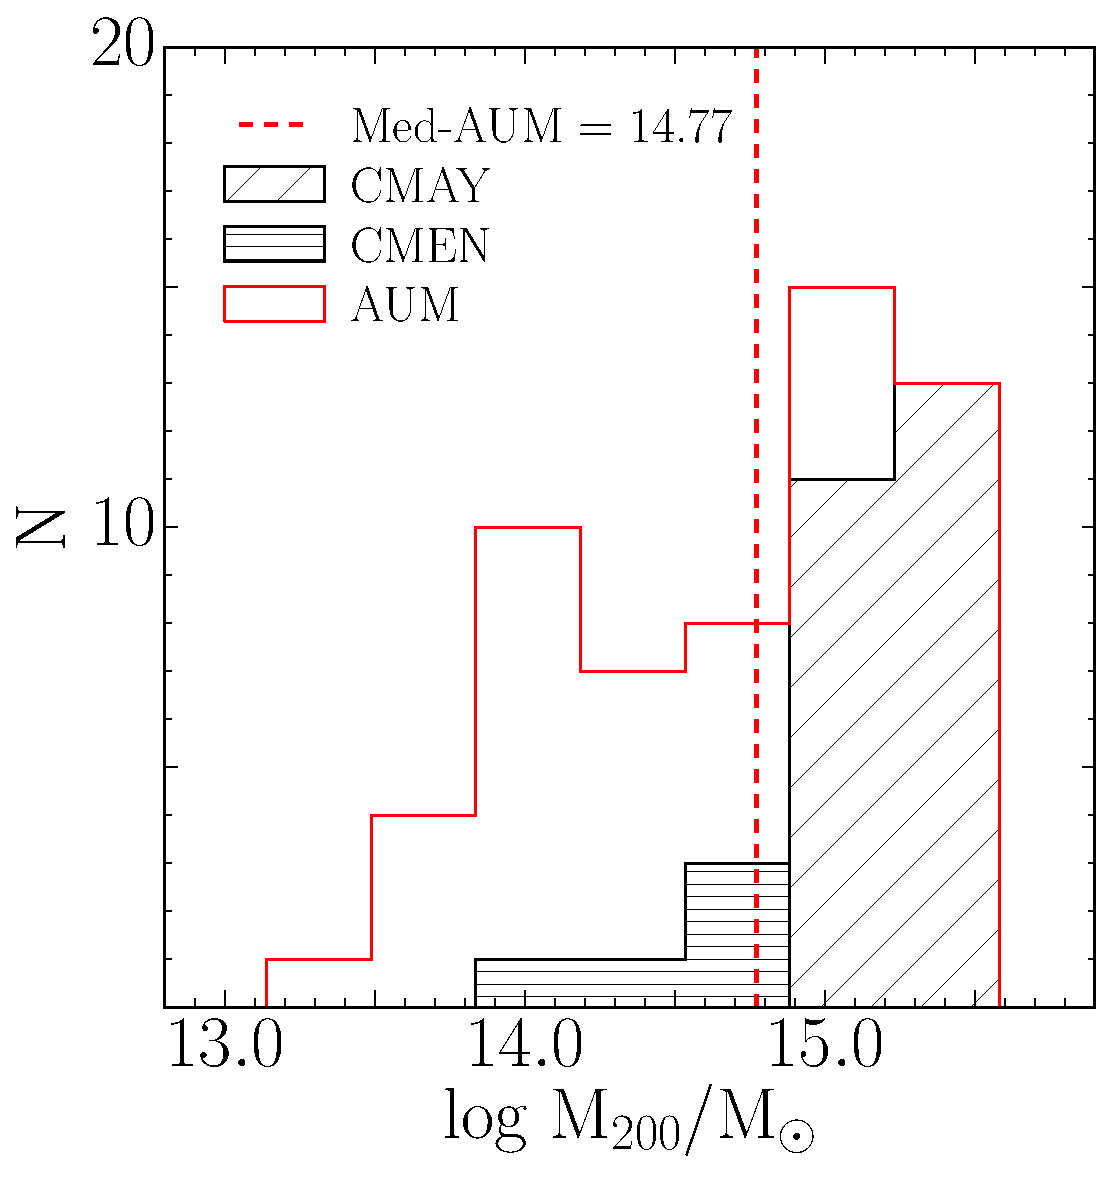
\includegraphics[height=9cm, width=9cm]{../al_final/LR/evolucion/histogramas/quilombo.pdf}
 \caption{La presete figure exhibe las distribuciones de masas M$_{200}$ de las muestras \cmay, \cmen y \aum}
 \label{fig:distribuciones}
\end{figure}


\section{Identificaci\'on de las BCGs}
El c\'odigo utilizado para realizar las simulaciones num\'ericas corre \textit{on the fly} un algoritmo {\it Friends-of-Friends} 
de identificaci\'on de halos (o c\'umulos de galaxias). Una vez identificado el c\'umulo, otro algoritmo corre sobre las part\'iculas que
forman parte del mismo para identificar sus subhalos (o galaxias sat\'elites) (Subfind, Dolag et al. 2009). Las part\'iculas de estrellas no 
ligadas a ninguna galaxia son asociadas por {\it Subfind} a la componente estelar del halo, formando as\'i un \'unico sistema BCG+Componente-Estelar-Difusa (o subhalo principal).

En este trabajo se considera que la part\'icula con m\'inimo de potencial del subhalo principal denota el centro de la BCG.
Para medir las masas de estas galaxias, tal es uno de los objetivos de este trabajo, se adoptar\'an diferentes aperturas centradas todas ellas, en el mencionado m\'inimo de potencial. 

\section{Medici\'on de la masa de las BCGs}
Observacionalmente, la obtenci\'on de las masas de las BCGs no es una medici\'on directa. El c\'alculo de la masa de las BCG se hace a
partir de una medici\'on de luminosidad y del posterior uso de un cociente masa-luminosidad.

Adem\'as de las diferentes asunciones para los cocientes masa-luminosidad utilizados, se pueden encontrar en la 
literatura diversas convenciones para medir la fotometr\'ia de las BCGs: magnitudes Petrosian, magnitudes tipo Kron, 
magnitudes obtenidas a partir de ajustes a los perfiles de brillo, magnitudes de apertura, magnitudes isofotales, 
magnitudes m\'etricas. A continuaci\'on se describen brevemente las utilizadas m\'as frecuentemente.

\begin{itemize}
\item Magnitudes Petrosian: La idea es medir una fracci\'on constante de la luz total independientemente de la distancia o posici\'on de la galaxia. Esta magnitud mide el flujo dentro del Radio Petrosian, el cual se calcula teniendo en cuenta el nivel de ruido de fondo y la forma del perfil de luz de la galaxia (Petrosian 1976; Blanton et al. 2001 y Yasuda et al. 2001). Es una medida robusta frente a variaciones de exposici\'on pero, seg\'un algunos estudios, no es apropiada para galaxias extendidas dado que subestima el flujo total. Por ejemplo seg\'un Blanton et al. 2001, la magnitud petrosian recupera casi todo el flujo para una galaxia disco pero s\'olo el $80\%$ para una galaxia con "bulge" con un perfil de de Vaucouleurs. Independientemente, Graham \& Driver (2005) encuentran que en la versi\'on utilizada por SLOAN (aperturas cirulares), la magnitud Petrosian subestima la luminosidad de galaxias con \'indices de Sersic $n=10$ en un $\sim45\%$ (0.64 mag). Bernardi et al. (2007) y Lauer et al. (2007) encuentran el mismo bias en galaxias BCGs.

\item Magnitudes Kron: Al igual que la anterior, se trata de una magnitud de "apertura escalada" en cuanto mide el flujo de la galaxia dentro de usualmente 2.5 radios de Kron. El radio de Kron se calcula teniendo en cuenta el perfil de luz (Kron 1980). No es tan robusta como la magnitud Petrosian en lo que respecta a variaciones exposici\'on-a-exposici\'on, pero es m\'as apropiada para medir el flujo total de las galaxias extendidas. Seg\'un Graham \& Driver (2005) una magnitud de Kron de una galaxia con bulge, con $n=4$, pierde $\sim 10\%$ del flujo. La dificultad para calcular esta magnitud reside en lograr una correcta medici/'on del radio de Kron, para hacerlo es necesario integrar el perfil de luz hasta radios relativamente grandes. Si la integraci\'on se corta incorrectamente el radio de Kron ser\'a mucho menor y por consiguiente se obtendr\'a un flujo equivocado, que puede llegar a ser hasta un $50\%$ menor que el real (Bernstein et al. 2002). Todos los trabajos que utilizan el software  mag\_auto de  SExtractor, calculan este tipo de magnitud (en aperturas el\'ipticas).

\item Magnitudes a partir de ajustes: En este caso hace falta ajustar alguna funci\'on al perfil de brillo de la galaxia. La magnitud de la galaxia se obtiene integrando el ajuste, en algunos casos truncando el fit en algún múltiplo del radio efectivo, en otros extrapolando a infinito. Un software muy usado en la literatura que trabaja de esta forma es GALFIT (Peng et al. 2010), el usuario puede elegir entre diferentes funciones de ajuste (Sersic, Moffat, King, Ferrer, etc.).  Bernardi+ 2013, Giallongo et al. 2014, Bellstedt+ 2016 son ejemplos de algunos trabajos en donde se usa GALFIT para obtener luminosidades de BCGs. Se pueden adem\'as encontrar trabajos en donde los autores obtienen las luminosidades de las BCGs haciendo sus propios ajustes (ej: Kravtsov et al. 2014, Gonzalez et al. 2005, Ascaso et al. 2011)

\item Magnitudes de apertura: Consiste simplemente en calcular magnitudes dentro de un radio fijo. Zhang et al. (2016) calculan por ejemplo magnitudes, y luego masas de BCGs, a partir de flujos medidos dentro de aperturas circulares de 15, 32, 50 y 60 kpc de radio.

\item Magnitudes Isofotales: Queda determinada por el flujo contenido dentro del radio donde el perfil de brillo superficial unidimensional alcanza un dado valor. Al igual que la magnitud de apertura, la magnitud isofotal posee la ventaja de ser insensible al modelo utilizado para ajustar el perfil de brillo, o a la forma del perfil de brillo. En el caso de las galaxias BCGs, esta propiedad resulta particularmente atractiva debido a la no universalidad del modelo que ajusta sus perfiles de brillo (ver \autoref{sec:perfiles}). 
Para citar algunos ejemplos, von der Linden et al. 2007 consideran que la BCG est\'a delmitada por un corte en $\mu_r=23~mag~arcsec^{-2}$ en la banda r. Fasano et al. 2010 usan el radio de la isofota $\mu_V=24~mag~arcsec^{-2}$ en la banda V. 




\end{itemize}
\section{Perfiles de brillo}
\label{sec:perfiles}
Varios trabajos pubicados recientemente han evidenciado que los perfiles de luz de algunas BCGs no pueden ser ajustados por una simple funci\'on de Sersic. 
Esto sucede cuando se verifica la presencia de una envolvente estelar extendida la cual habr\'ia sido acumulada en la parte externa de la BCG a lo largo de su formaci\'on (residuos de "mergers" o "stripping" de material de otras galaxias).

Para poder ajustar los perfiles de luz de estas galaxias extendidas hace falta sumar a la funci\'on de Sersic una componente externa, la cual puede ser otra funci\'on de Sersic o una funci\'on Exponencial (ej: Seigar et al. 2007; Donzelli et al. 2011; Ascaso et al. 2011). 

\subsection{Relaci\'on de Kormendy}
Ascaso et al. 2011 estudian una muestra de BCG a z bajo ($0.04<z<0.07$) y comparan con otra a z intermedio $0.3<z<0.6$. Encuentran que la pendiente de la relaci\'on de Kormendy crece hacia z bajos pasando de 3.3 a 4.2. Bildfell et al. 2008 tambi\'en encuentran el mismo comportamiento al comparar una muestra de BCGs a $0.15<z<0.55$  con otra local.

(Las medianas de $mu_e$ y $r_e$ en las muestras de Ascaso et al. 2011 muestran que el cambio en $mu_e$ no es significativo pero s\'i el cambio en $r_e$.)

\subsection{Par\'ametros estructurales vs. MasaBCG}
Ascaso et al. 2011 estudian  la relaci\'on existente entre las magnitudes absolutas de sus dos muestras con $n$, $r_e$ y $mu_e$. Encuentran que a una dada luminosidad las BCGs m\'as cercanas tienen $mu_e$ m\'as d\'ebil, $r_e$ m\'as grandes y par\'ametros de Sersic similares que las BCGs de la muestra a redshift intermedio.


%------------------------------------------------
%------------------------------------------------
 \section{Grasil 3D.... }

%\lipsum[6]

%----------------------------------------------------------------------------------------

% Chapter 4

\chapter{Resultados} % Chapter title

\label{ch:resultados} % For referencing the chapter elsewhere, use \autoref{ch:mathtest}

%----------------------------------------------------------------------------------------


\section{La importancia del AGN en los modelos de formaci\'on de galaxias}
Uno de los desaf\'ios actuales al cual se enfrentan los modelos de formaci\'on de galaxias, en lo que 
respecta a las galaxias masivas, consiste en controlar el excesivo enfriamento del gas para as\'i evitar tasas 
de formaci\'on estelar por encima de los valores que se observan en el Universo. En la actualidad, se sabe que los 
c\'alculos efectuados sin incluir una inhibici\'on eficiente al ensamblaje de la masa estelar en el rango de masas altas 
de la funci\'on de masa, donde el feedback de supernovas se vuelve ineficiente, lleva a una sobre predicci\'on de la masa 
estelar en estos sistemas por un factor $\sim$10 (ej, Benson et al. 2003).

El {\it feedback} de supernovas, utilizado en los modelos para controlar la formaci\'on estelar en galaxias,
deja de ser eficiente en aquellas m\'as masivas, en particular en las BCGs, en donde una fuente adicional de calentamiento 
para el gas se hace necesaria, siendo la soluci\'on m\'as prometente el {\it feedback} proveniente de la actividad AGN.

Sorprendentemente, este proceso f\'isico ha sido ignorando en los c\'alculos presentes en los modelos de formaci\'on de galaxias durante
mucho tiempo. Sin embargo, desde hace aproximadamente una d\'ecada, su uso en modelos semianal\'iticos 
y en simumlaciones num\'ericas hidrodin\'amicas, ha crecido progresivamente 
(ej. Granato et al. 2004; Springel, Di Matteo $\&$ Hernquist 2005; Bower et al. 2006; Croton et al. 2006; Monaco,
Fontanot $\&$ Taffoni 2007; Sijacki et al. 2007; Somerville et al. 2008; Fabjan et al. 2010; McCarthy et al. 2010;
Martizzi, Teyssier $\&$ Moore 2012; Ragone-Figueroa et al. 2013; Dubois et al. 2014, Martizzi et al. 2016; Bah\'e et al. 2017;
Pillepich et al. 2017).

En el campo de las simulaciones num\'ericas, el uso del {\it feedback} de AGN reduce la masa estelar de las galaxias BCGs
en un factor que var\'ia de 2 a 10 dependiendo del modelo y de la masa de la galaxia considerada (Sijacki et al. 2007; Martizzi 
et al. 2012; Stott et al. 2012; Dubois et al. 2013; Ragone-Figueroa et al. 2013). No obstante, como se ver\'a en \ref{sec:zeta0} el contenido 
estelar de estas galaxias simuladas sigue siendo alto comparado con las masas que miden las observaciones.


En la Fig.
%~\ref{fig:} XXXX 
puede verse el impacto del modelo de {\it feedback} de AGN usado en estas simulaciones sobre las
masas finales (a $z=0$) de dos BCGs y sus respectivos c\'umulos, uno en la muestra de alta masa y otro en la muestra de baja masa. 
En ambos casos la disminuci\'on de la masa final al encender el AGN en la simulaci\'on es evidente.


\begin{figure}[H]
 \hspace*{-0.5cm}
 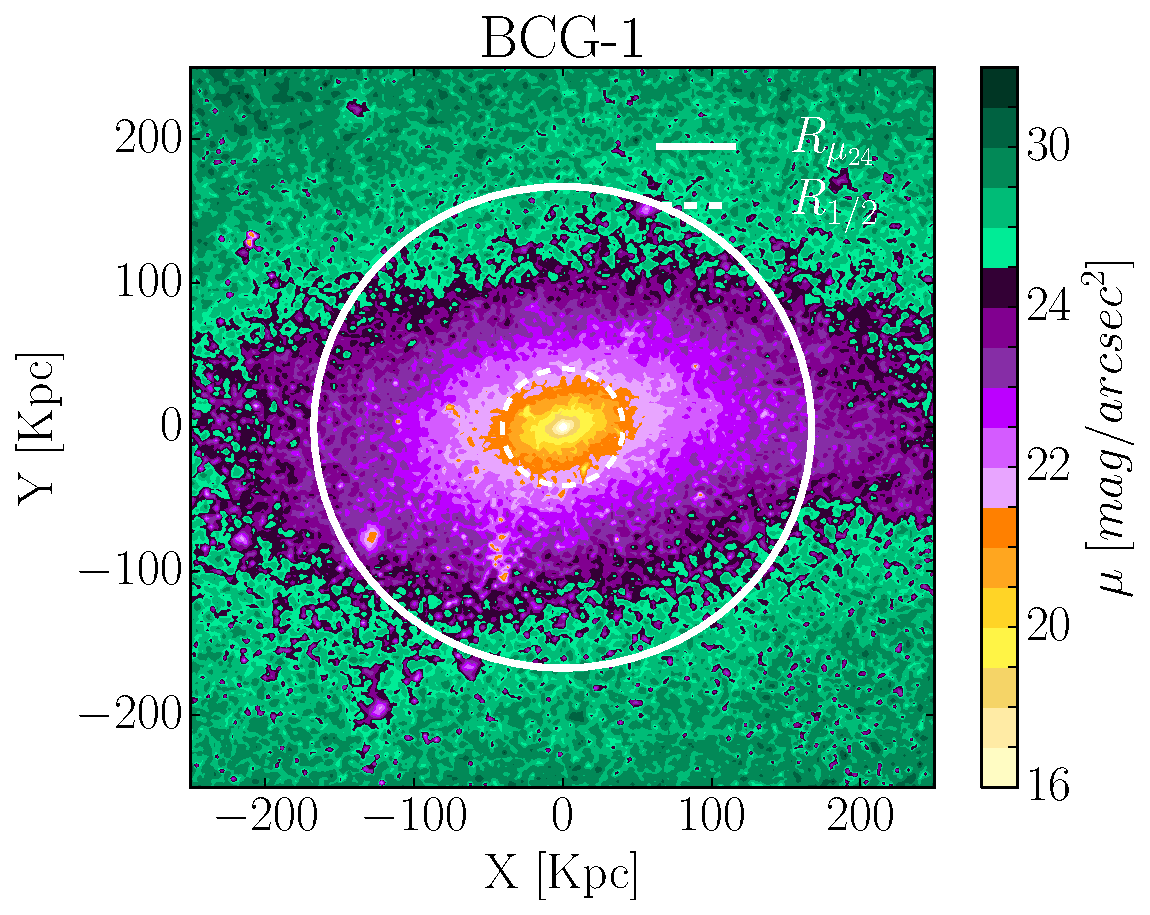
\includegraphics[height=7cm, width=9.0cm, trim={0cm 2.1cm 3.3cm 1cm},clip]{../al_final/LR/LR_CSF/nodust/grupo0/mu24/D1/091/maps_D1_aperturas.pdf}
 \hspace*{-0.27cm}
 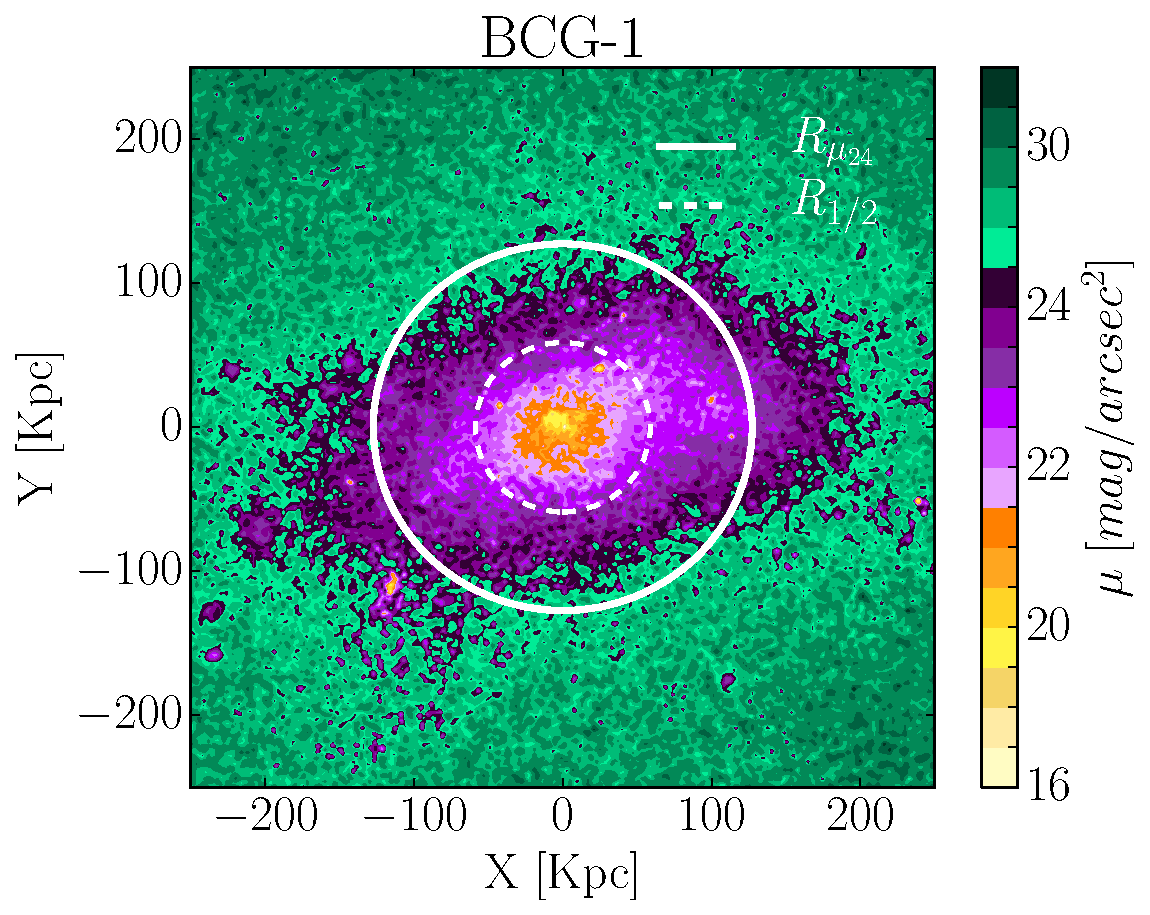
\includegraphics[height=7cm, width=9.0cm, trim={3.2cm 2.1cm 0cm 1cm},clip]{../al_final/LR/LR_minpot3_rmmax/nodust/grupo0/mu24/D1/091/maps_D1_aperturas.pdf}
 \\
  \hspace*{-0.5cm}
 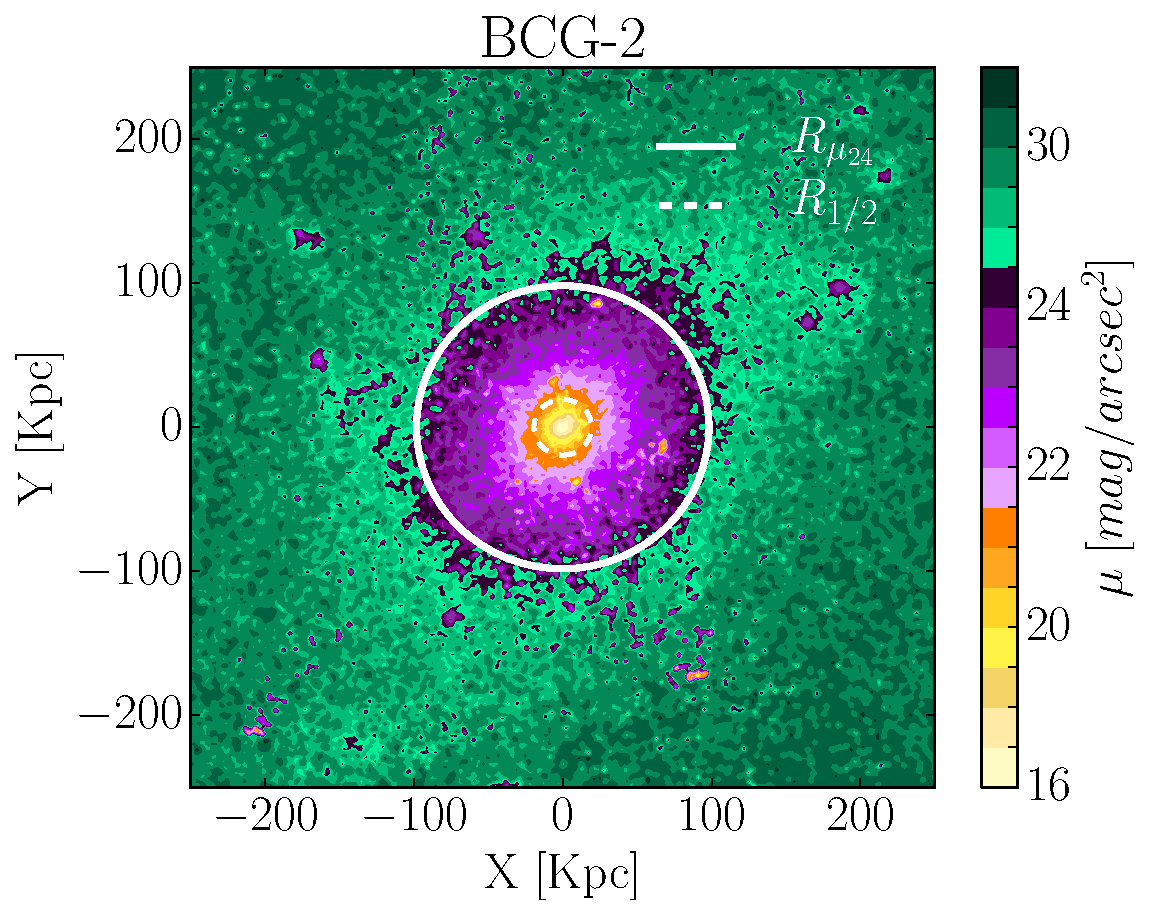
\includegraphics[height=8cm, width=9.0cm, trim={0cm 0cm 3.3cm 1.1cm},clip]{../al_final/LR/LR_CSF/nodust/grupo0/mu24/D2/091/maps_D2_aperturas.pdf}
 \hspace*{-0.27cm}
 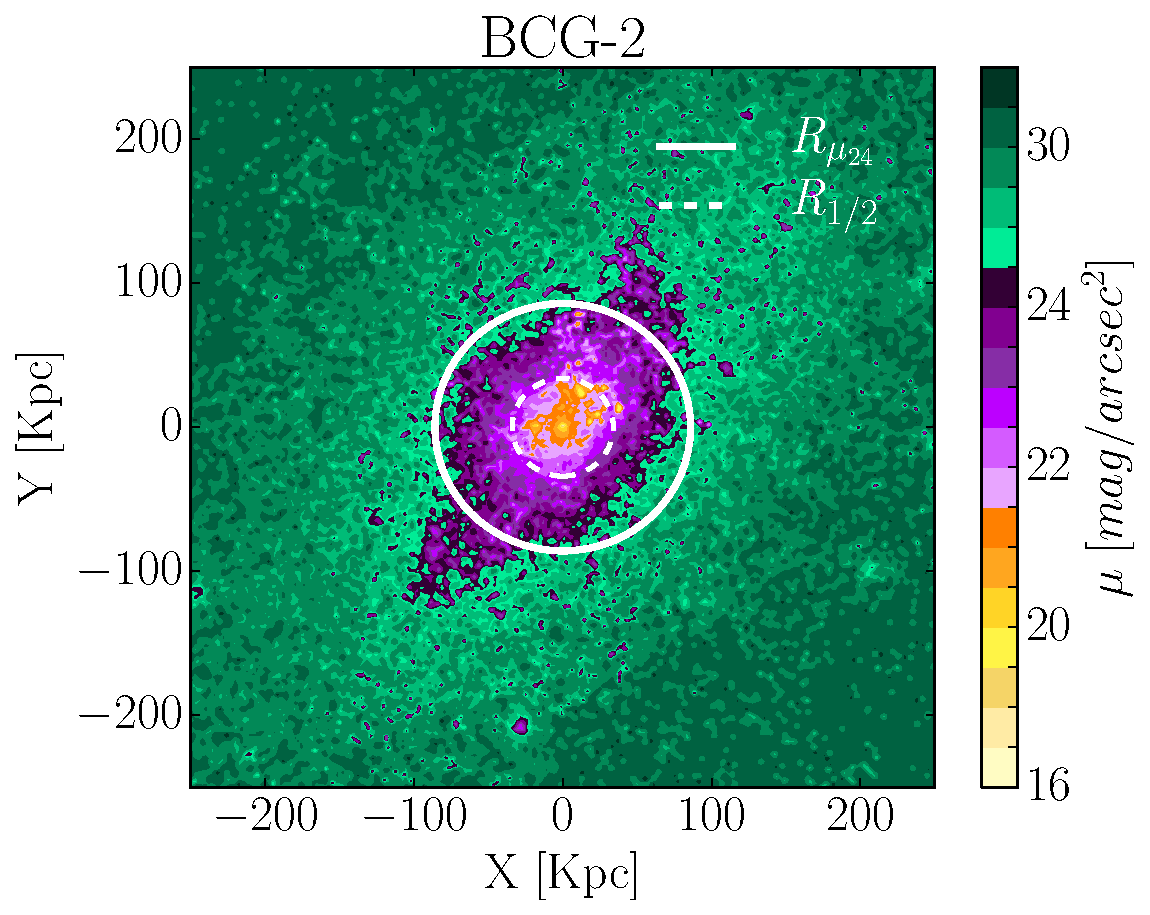
\includegraphics[height=8cm, width=9.0cm, trim={3.2cm 0cm 0cm 1.1cm},clip]{../al_final/LR/LR_minpot3_rmmax/nodust/grupo0/mu24/D2/091/maps_D2_aperturas.pdf}
\caption[csfagnmap]{}
\end{figure}



\begin{figure}[H]
 \centering
 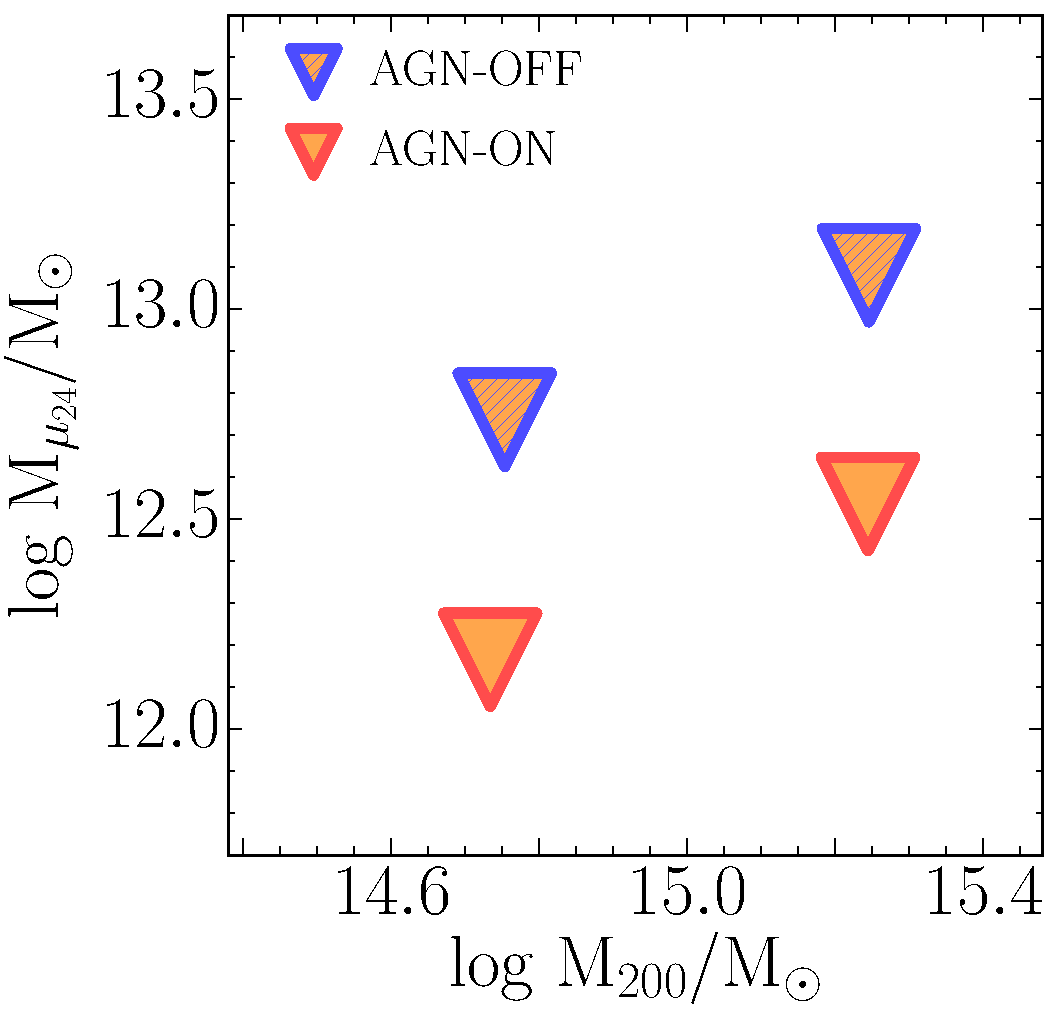
\includegraphics[height=8cm, width=9cm]{../al_final/LR/evolucion/relaciones/csf_agn.pdf}
\end{figure}

\begin{figure}[H]
 \centering
 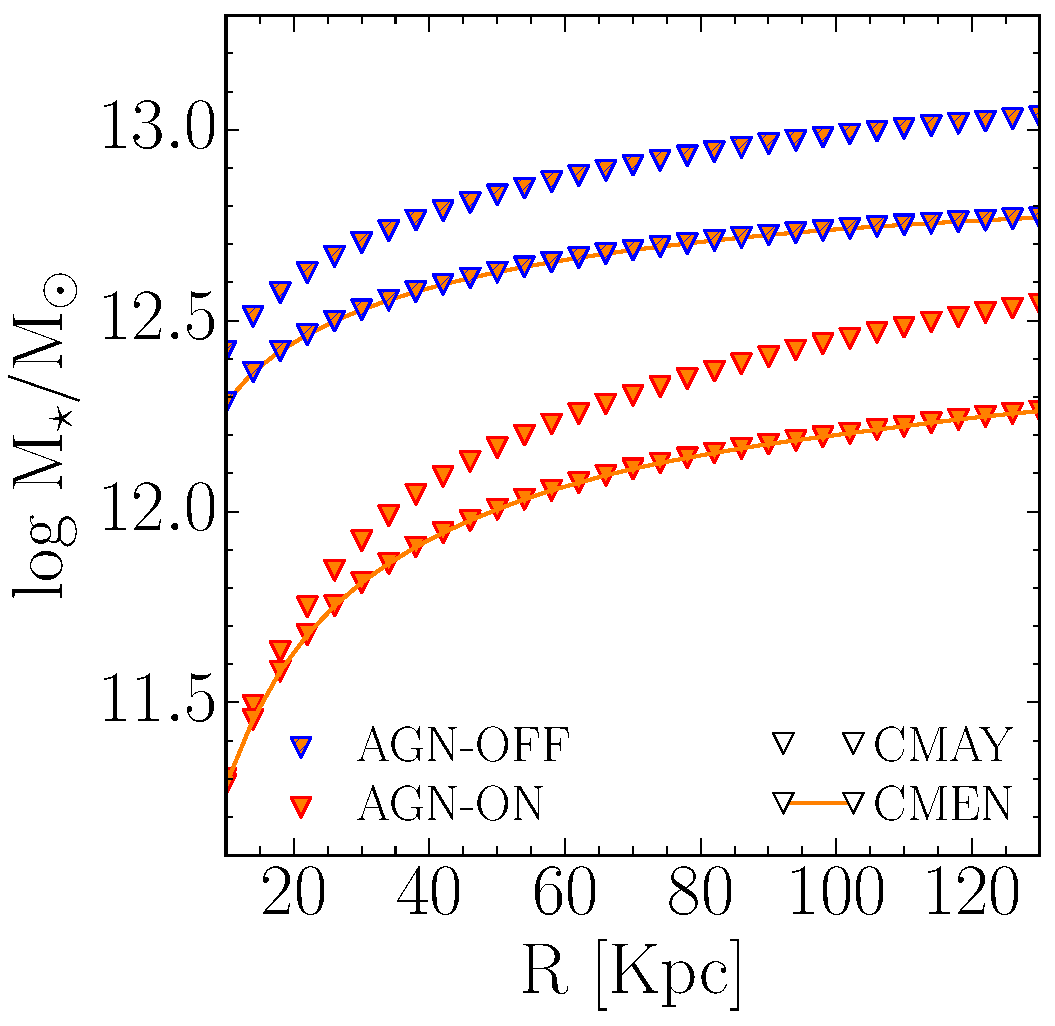
\includegraphics[height=8cm, width=9cm]{../al_final/LR/evolucion/relaciones/csf_agn_acumuladas.pdf}
 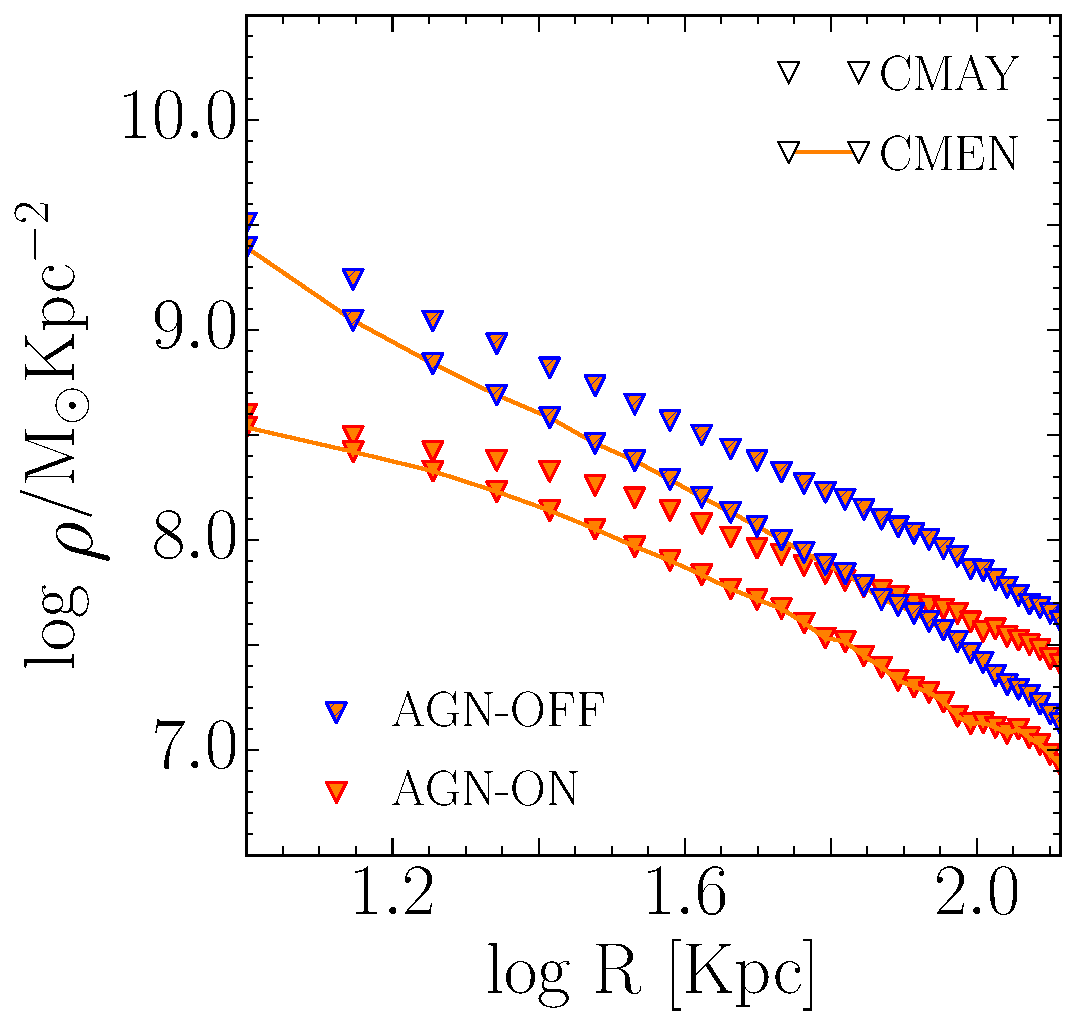
\includegraphics[height=8cm, width=9cm]{../al_final/LR/evolucion/relaciones/csf_agn_perfil_dens_masa_con_log.pdf}
\end{figure}


\section{Masas de la BCG en funci\'on de la apertura}

%la mas excentrica
\begin{figure}[H]
 \centering
 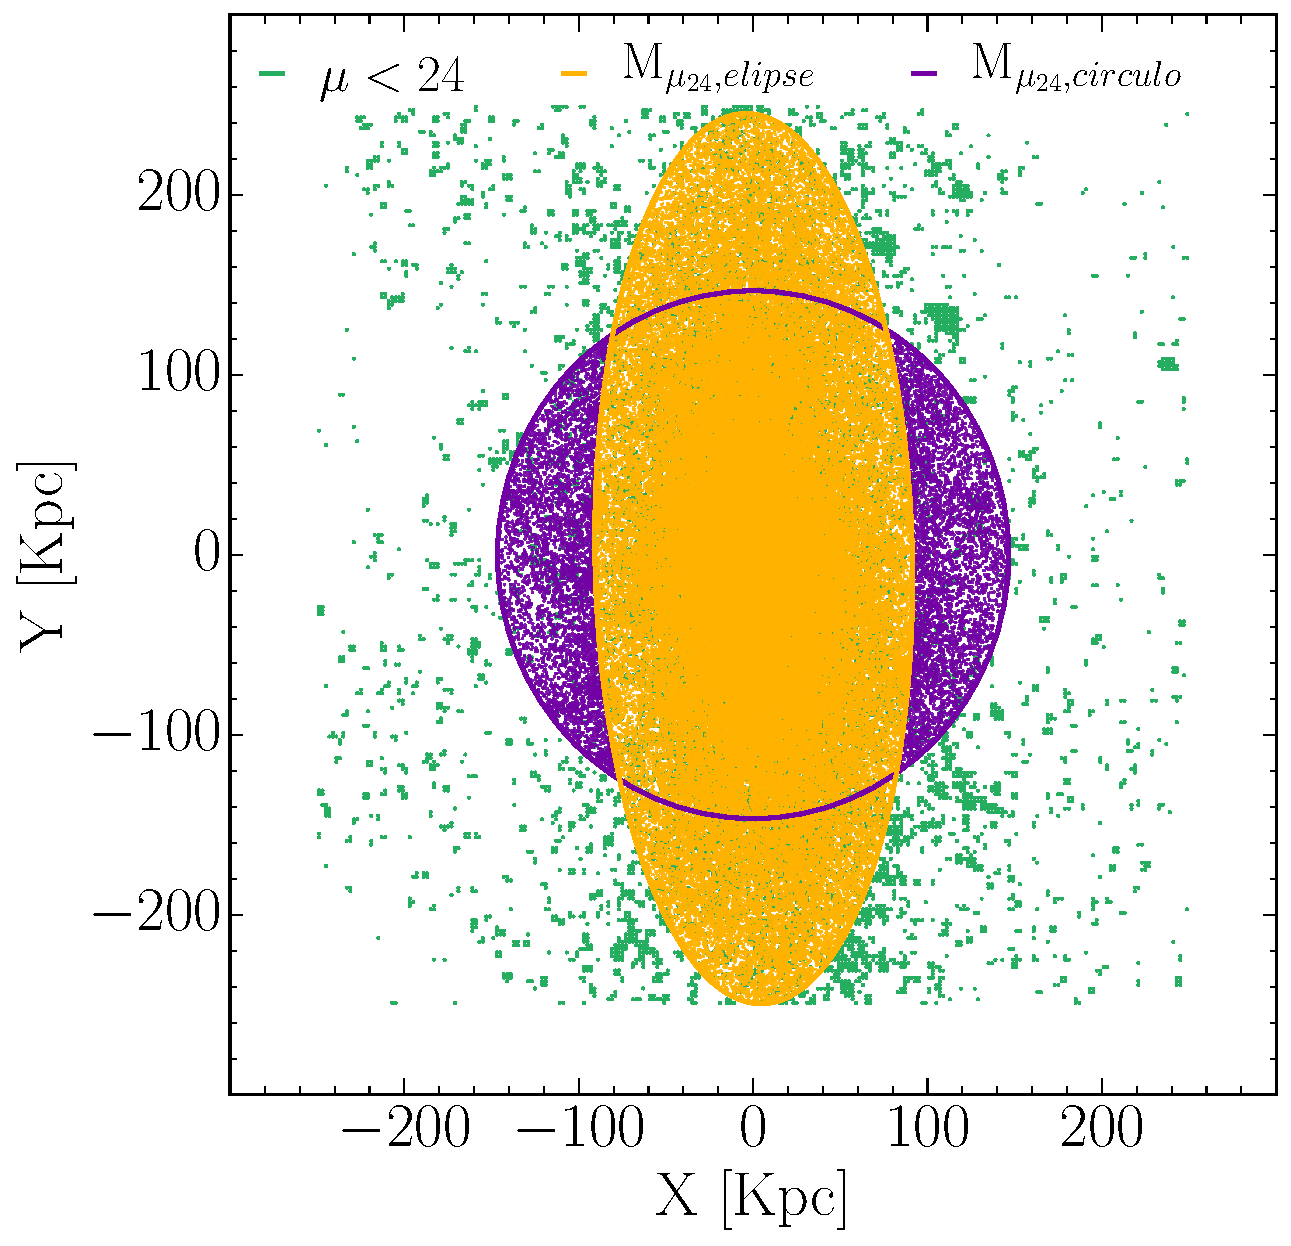
\includegraphics[height=9cm, width=9cm]{../al_final/plots/elipses/D22elipse-circ.pdf}
\end{figure}

\begin{figure}[H]
 \centering
 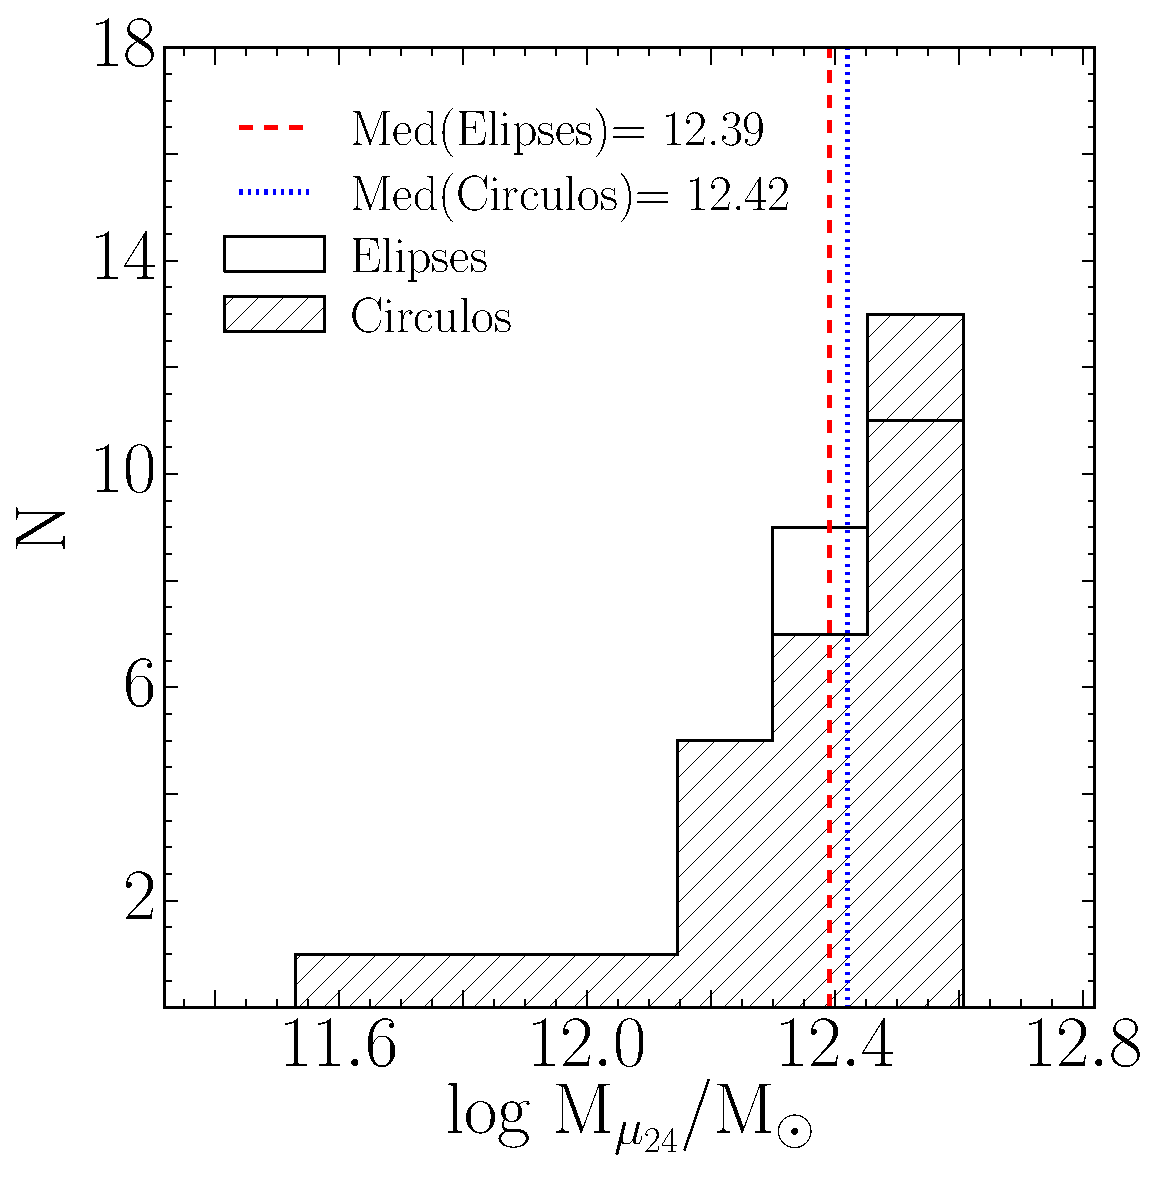
\includegraphics[height=9cm, width=9cm]{../al_final/LR/evolucion/histogramas/Mmu_elipse_vs_circ.pdf}
\end{figure}

\section{BCGs z=0}


\begin{tabular}{c c c c c}
\hspace*{-1cm} 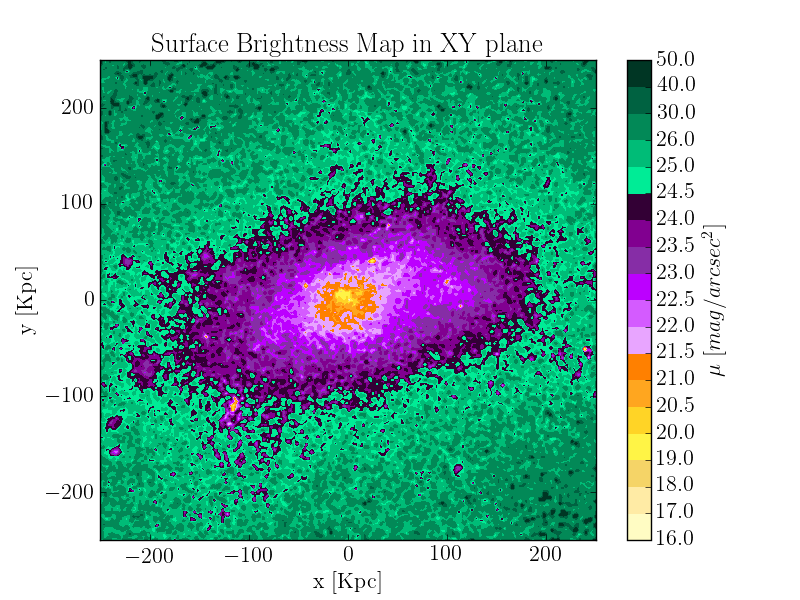
\includegraphics[height=4cm,width=4cm,trim={2.5cm 1.5cm 5cm 1.5cm},clip]{../pngs/D1.png}  & 
 \hspace*{-0.3cm}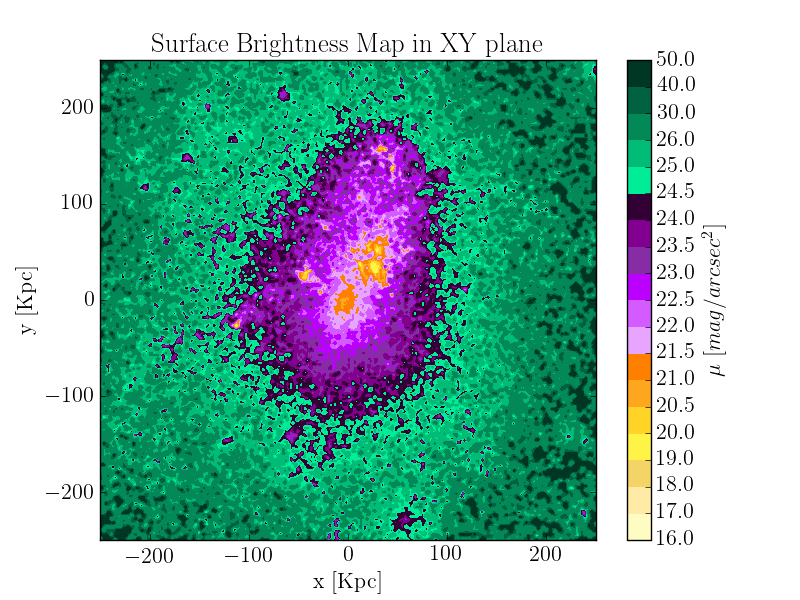
\includegraphics[height=4cm,width=4cm,trim={2.5cm 1.5cm 5cm 1.5cm},clip]{../pngs/D6.png}  & 
 \hspace*{-0.3cm}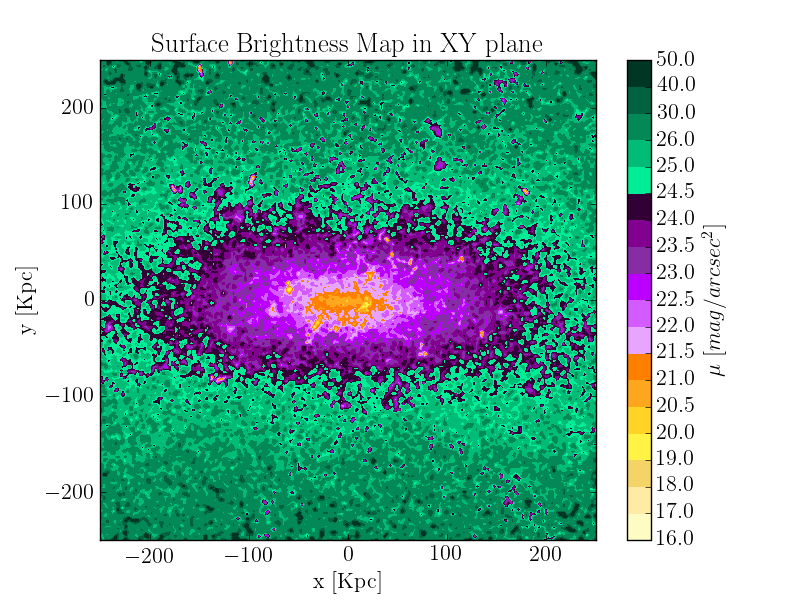
\includegraphics[height=4cm,width=4cm,trim={2.5cm 1.5cm 5cm 1.5cm},clip]{../pngs/D7.png}  & 
 \hspace*{-0.3cm}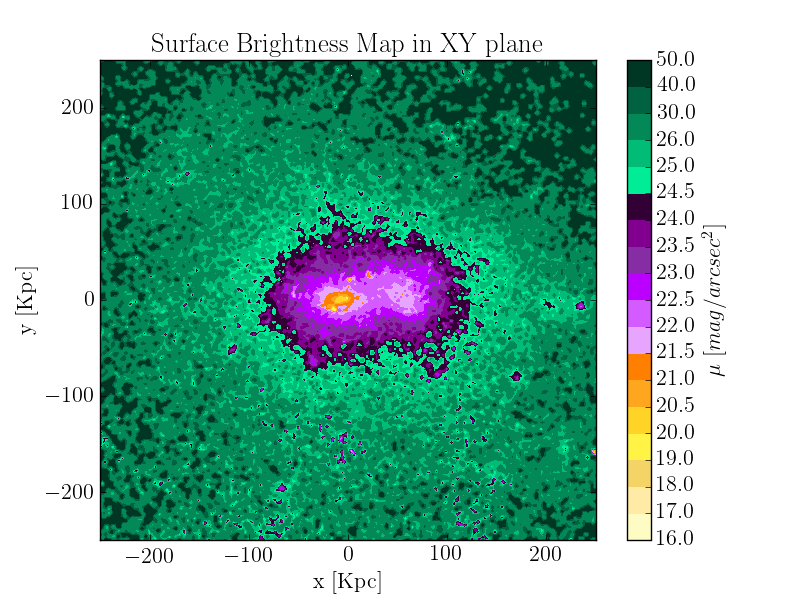
\includegraphics[height=4cm,width=4cm,trim={2.5cm 1.5cm 5cm 1.5cm},clip]{../pngs/D8.png}  & 
  \hspace*{-0.3cm}\multirow{6}{*}
  {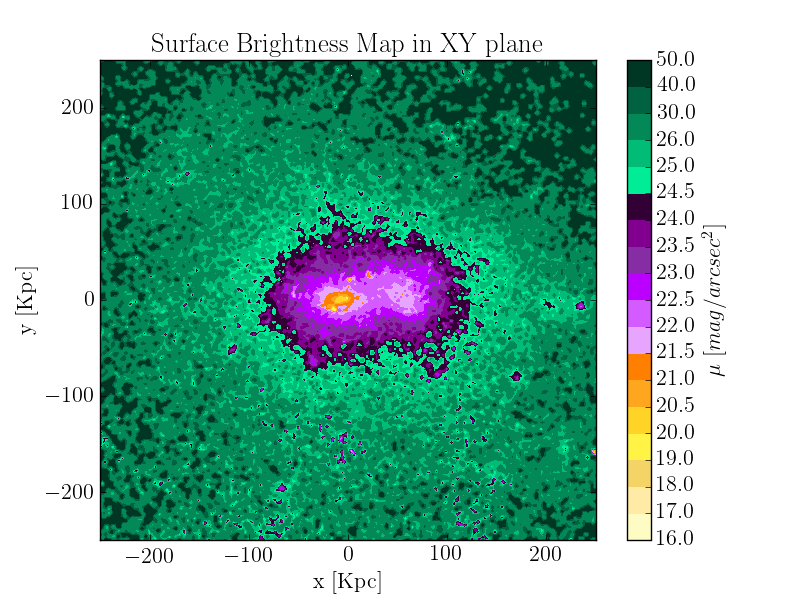
\includegraphics[height=15cm,width=3cm,trim={15.5cm 1.cm 0cm 1.cm},clip]{../pngs/D8.png}}
 \\

 \hspace*{-1cm}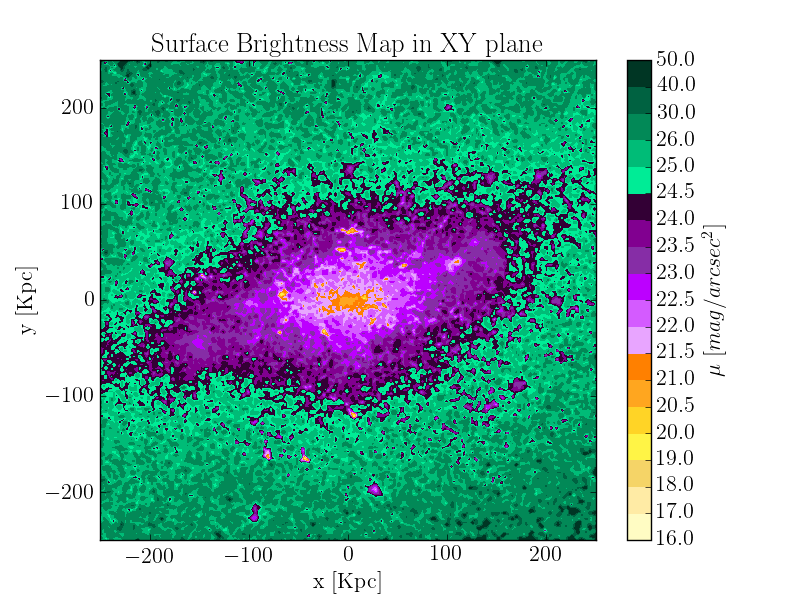
\includegraphics[height=4cm,width=4cm,trim={2.5cm 1.5cm 5cm 1.5cm},clip]{../pngs/D10.png}  & 
 \hspace*{-.3cm}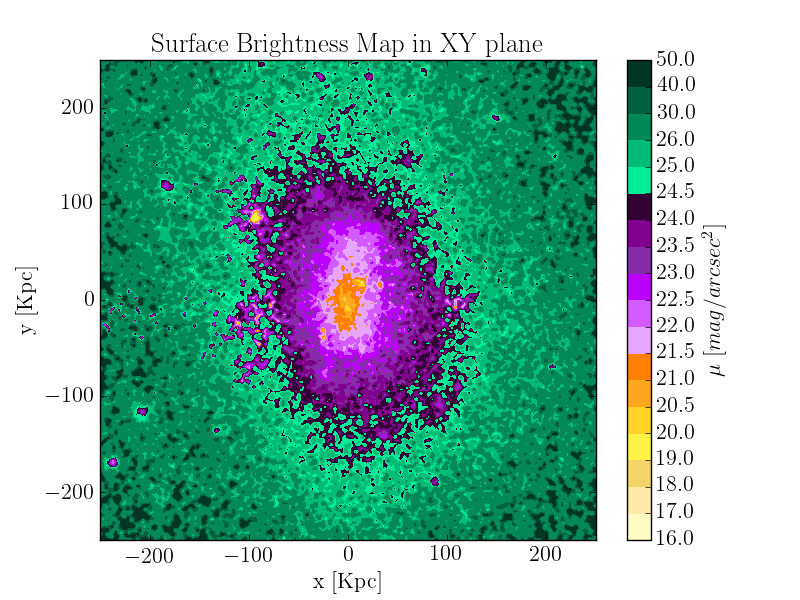
\includegraphics[height=4cm,width=4cm,trim={2.5cm 1.5cm 5cm 1.5cm},clip]{../pngs/D11.png}  & 
 \hspace*{-.3cm}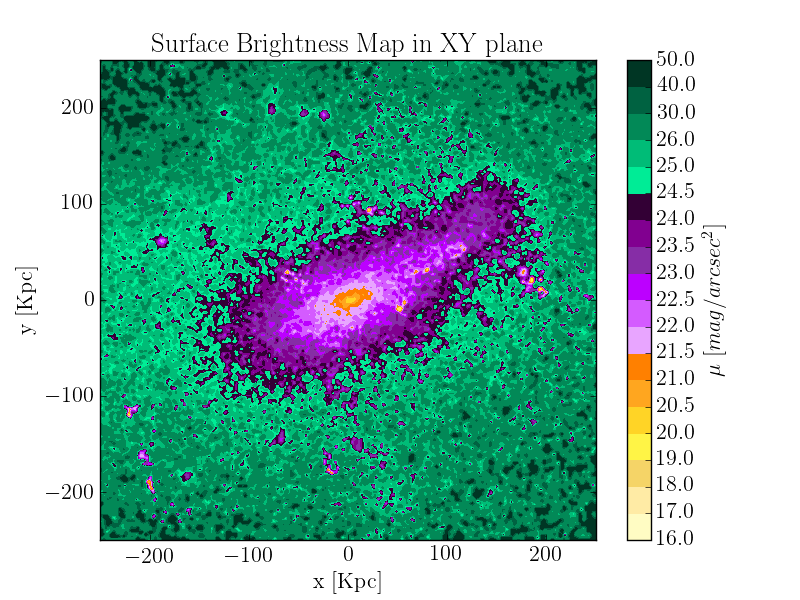
\includegraphics[height=4cm,width=4cm,trim={2.5cm 1.5cm 5cm 1.5cm},clip]{../pngs/D12.png}  & 
 \hspace*{-.3cm}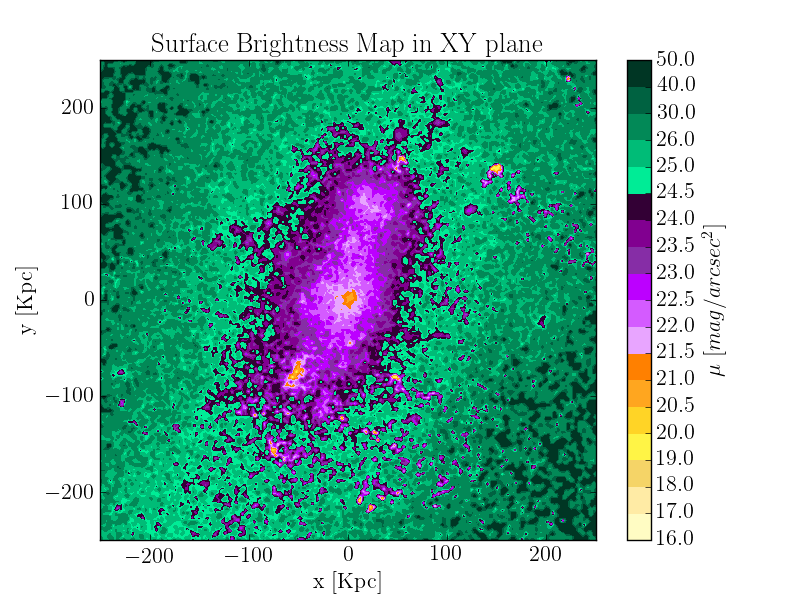
\includegraphics[height=4cm,width=4cm,trim={2.5cm 1.5cm 5cm 1.5cm},clip]{../pngs/D13.png}  &
 \\

 \hspace*{-1cm}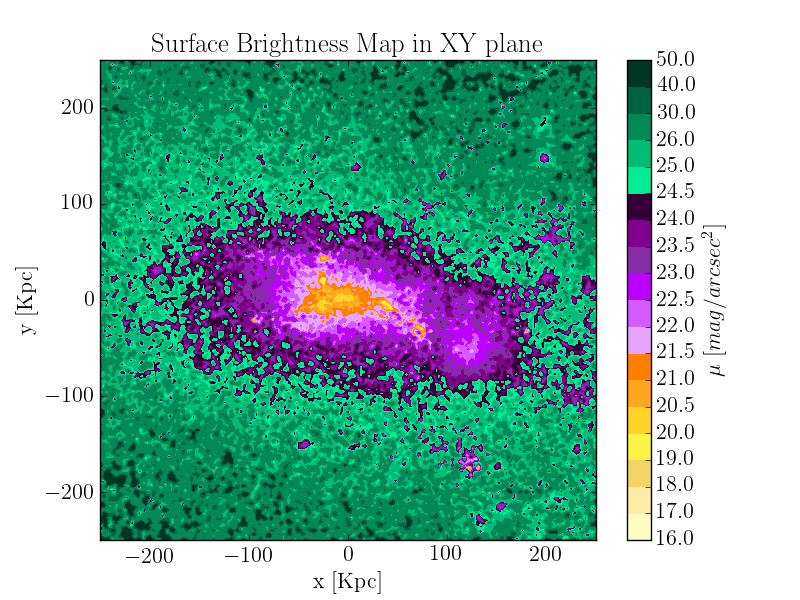
\includegraphics[height=4cm,width=4cm,trim={2.5cm 1.5cm 5cm 1.5cm},clip]{../pngs/D14.png}  & 
 \hspace*{-.3cm}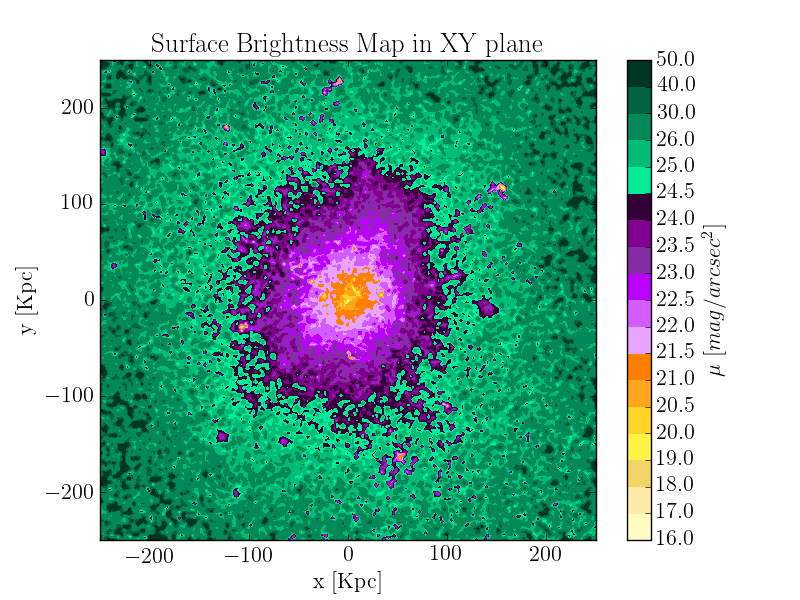
\includegraphics[height=4cm,width=4cm,trim={2.5cm 1.5cm 5cm 1.5cm},clip]{../pngs/D15.png}  & 
 \hspace*{-.3cm}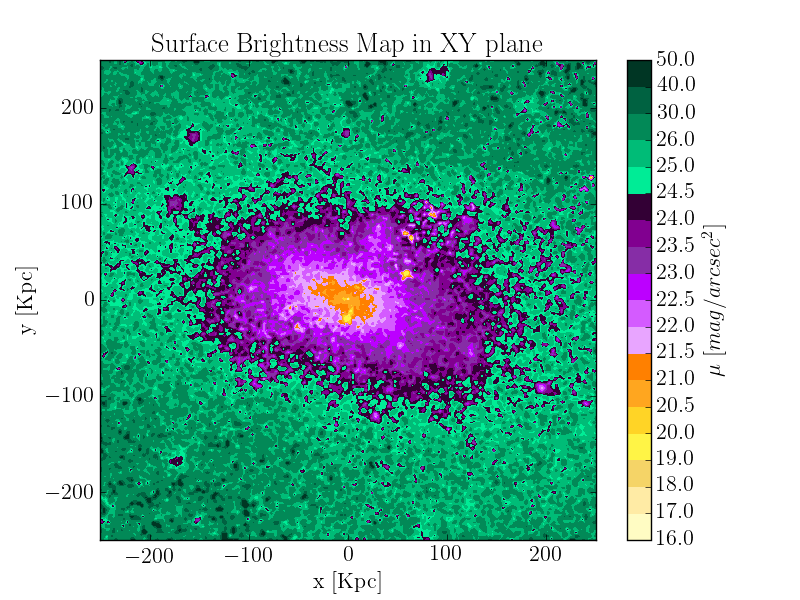
\includegraphics[height=4cm,width=4cm,trim={2.5cm 1.5cm 5cm 1.5cm},clip]{../pngs/D16.png}  & 
 \hspace*{-.3cm}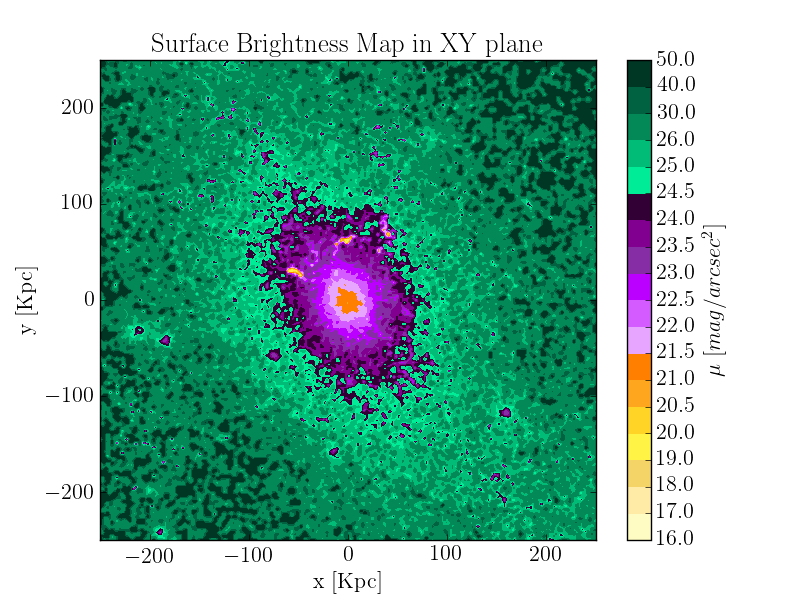
\includegraphics[height=4cm,width=4cm,trim={2.5cm 1.5cm 5cm 1.5cm},clip]{../pngs/D17.png}  &
 \\ 

 \hspace*{-1cm}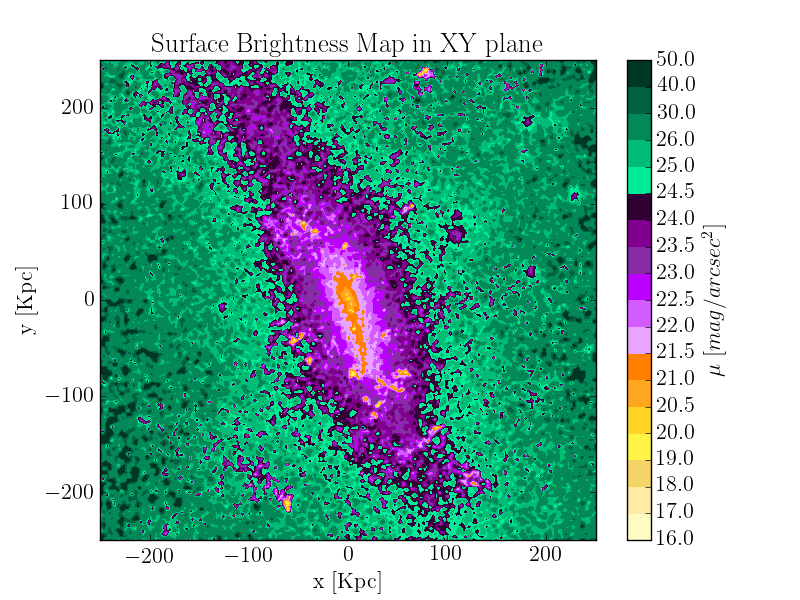
\includegraphics[height=4cm,width=4cm,trim={2.5cm 1.5cm 5cm 1.5cm},clip]{../pngs/D18.png}  & 
 \hspace*{-.3cm}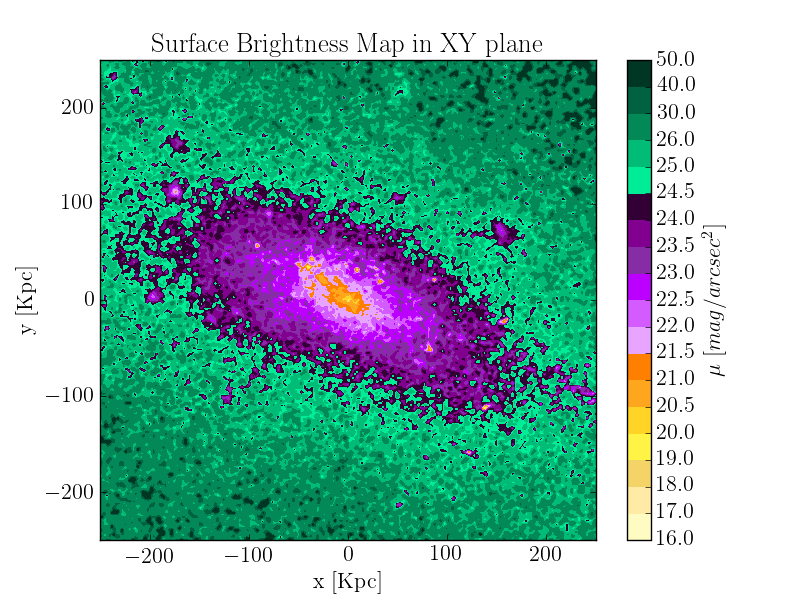
\includegraphics[height=4cm,width=4cm,trim={2.5cm 1.5cm 5cm 1.5cm},clip]{../pngs/D19.png}  & 
 \hspace*{-.3cm}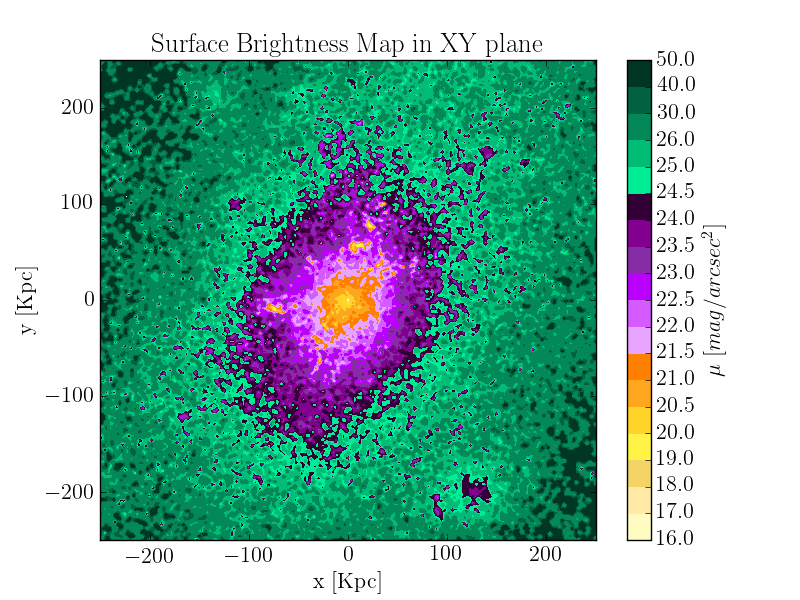
\includegraphics[height=4cm,width=4cm,trim={2.5cm 1.5cm 5cm 1.5cm},clip]{../pngs/D20.png}  & 
 \hspace*{-.3cm}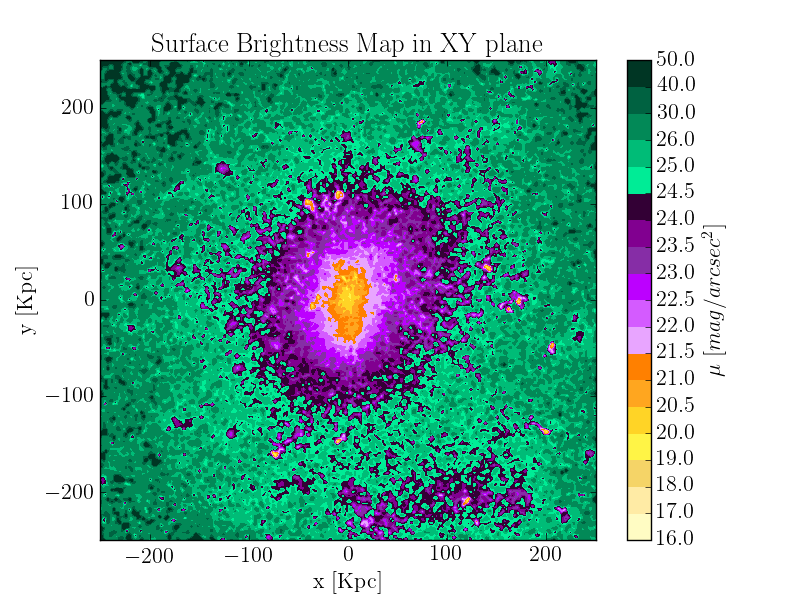
\includegraphics[height=4cm,width=4cm,trim={2.5cm 1.5cm 5cm 1.5cm},clip]{../pngs/D21.png}  &
 \\ 

 \hspace*{-1cm}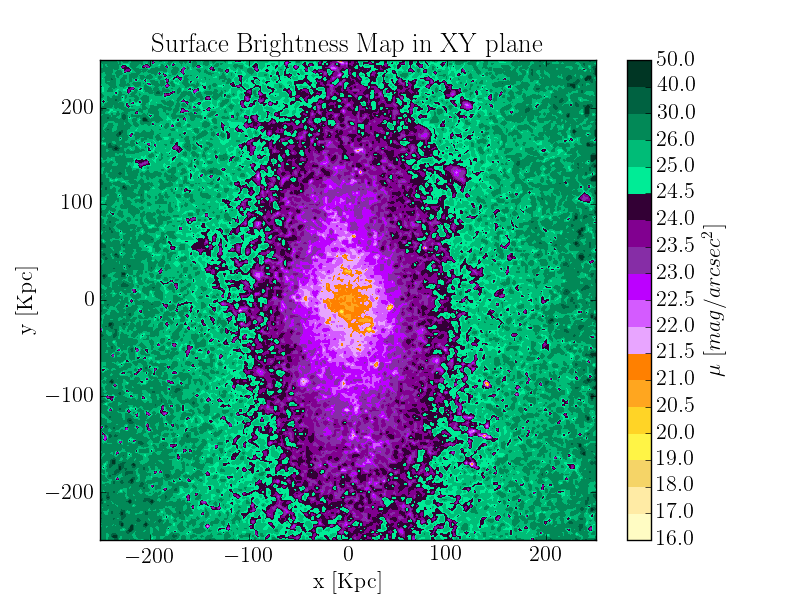
\includegraphics[height=4cm,width=4cm,trim={2.5cm 1.5cm 5cm 1.5cm},clip]{../pngs/D22.png}  & 
 \hspace*{-.3cm}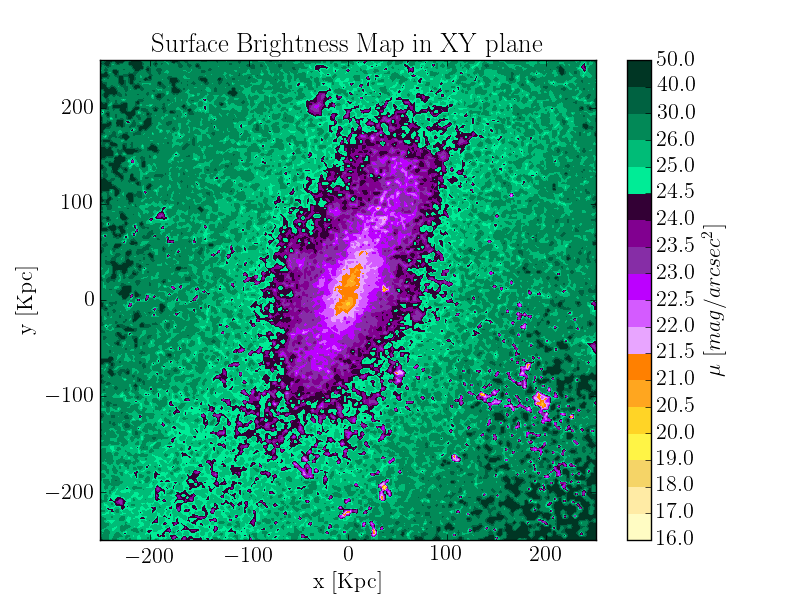
\includegraphics[height=4cm,width=4cm,trim={2.5cm 1.5cm 5cm 1.5cm},clip]{../pngs/D23.png}  & 
 \hspace*{-.3cm}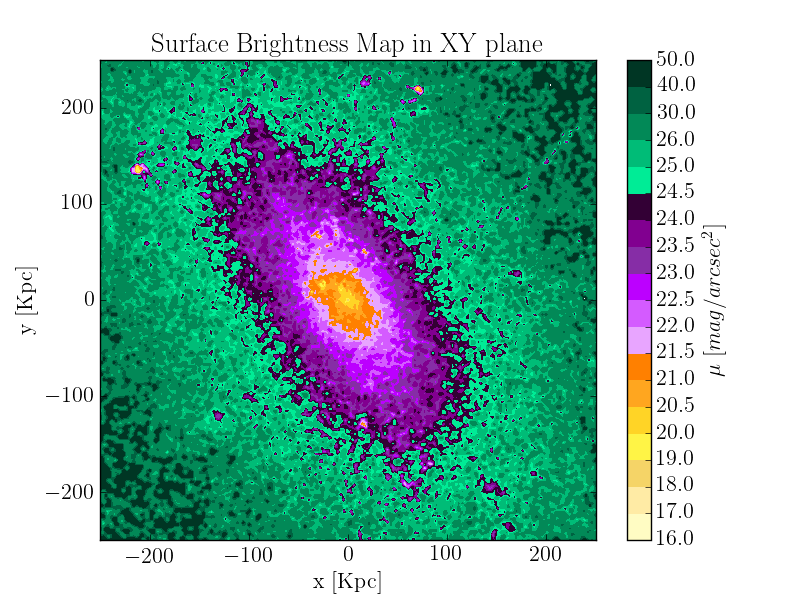
\includegraphics[height=4cm,width=4cm,trim={2.5cm 1.5cm 5cm 1.5cm},clip]{../pngs/D24.png}  & 
 \hspace*{-.3cm}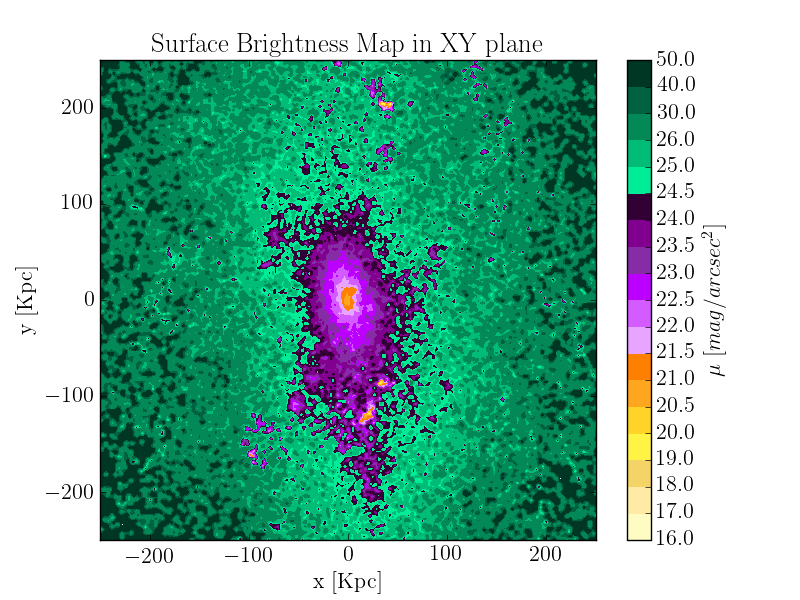
\includegraphics[height=4cm,width=4cm,trim={2.5cm 1.5cm 5cm 1.5cm},clip]{../pngs/D25.png}  &
 \\ 

 \hspace*{-1cm}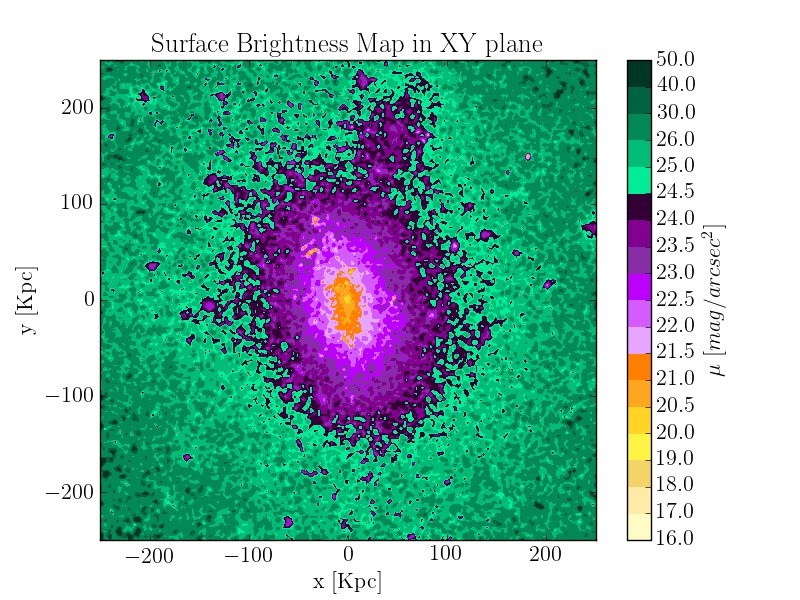
\includegraphics[height=4cm,width=4cm,trim={2.5cm 1.5cm 5cm 1.5cm},clip]{../pngs/D26.png}  & 
 \hspace*{-.3cm}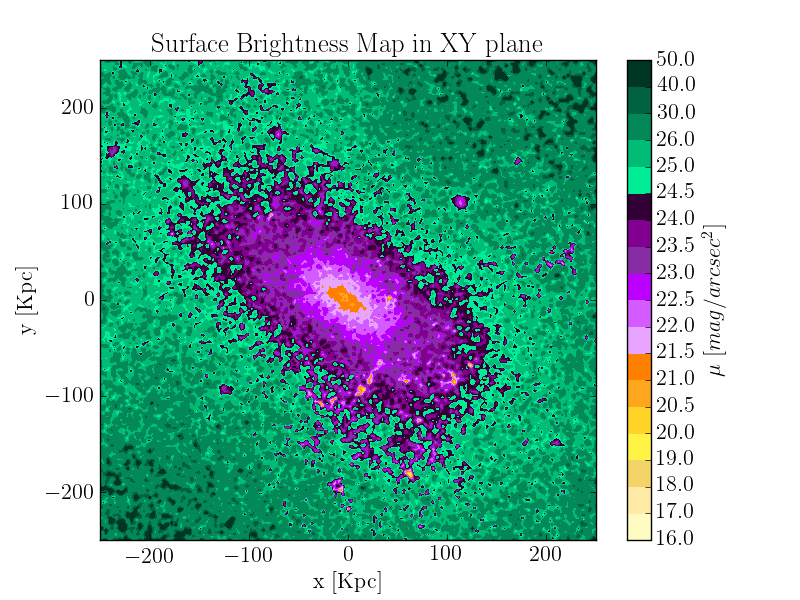
\includegraphics[height=4cm,width=4cm,trim={2.5cm 1.5cm 5cm 1.5cm},clip]{../pngs/D27.png}  & 
 \hspace*{-.3cm}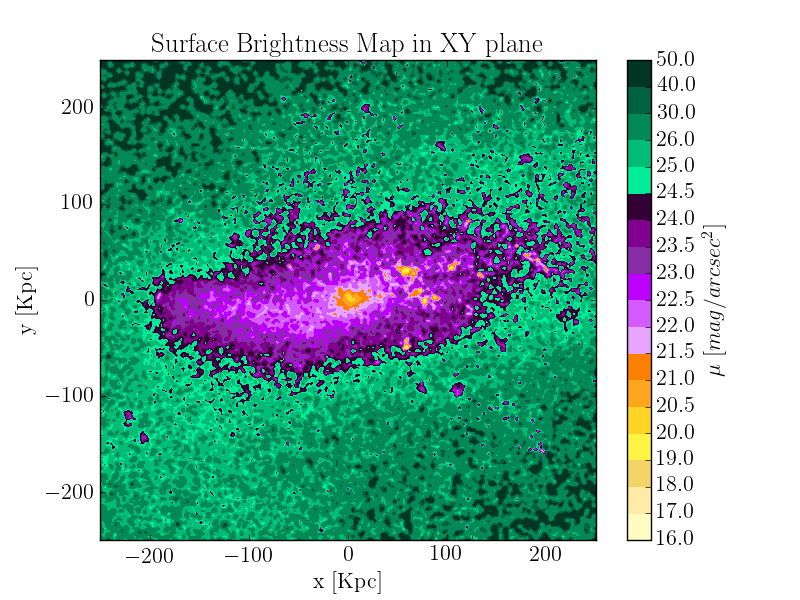
\includegraphics[height=4cm,width=4cm,trim={2.5cm 1.5cm 5cm 1.5cm},clip]{../pngs/D28.png}  & 
 \hspace*{-.3cm}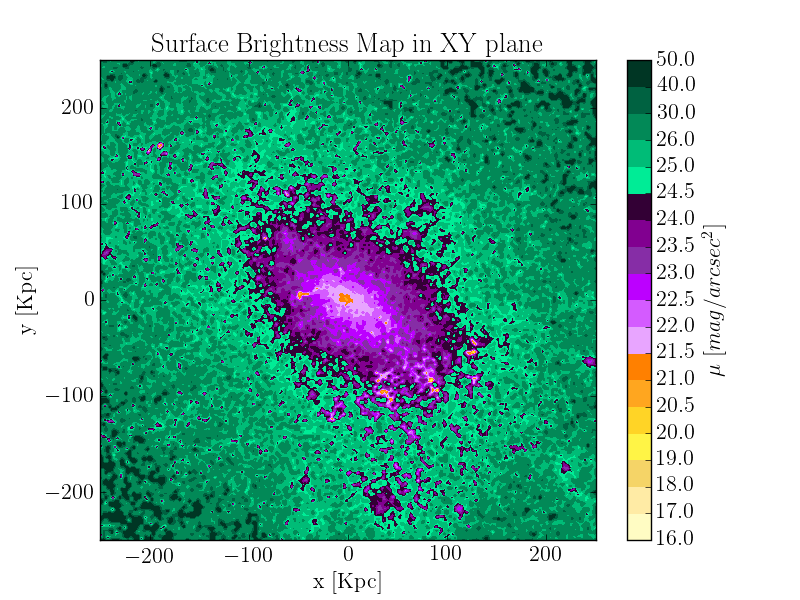
\includegraphics[height=4cm,width=4cm,trim={2.5cm 1.5cm 5cm 1.5cm},clip]{../pngs/D29.png}  &
 \\
 
\end{tabular}


\begin{figure}[H]
 \centering
 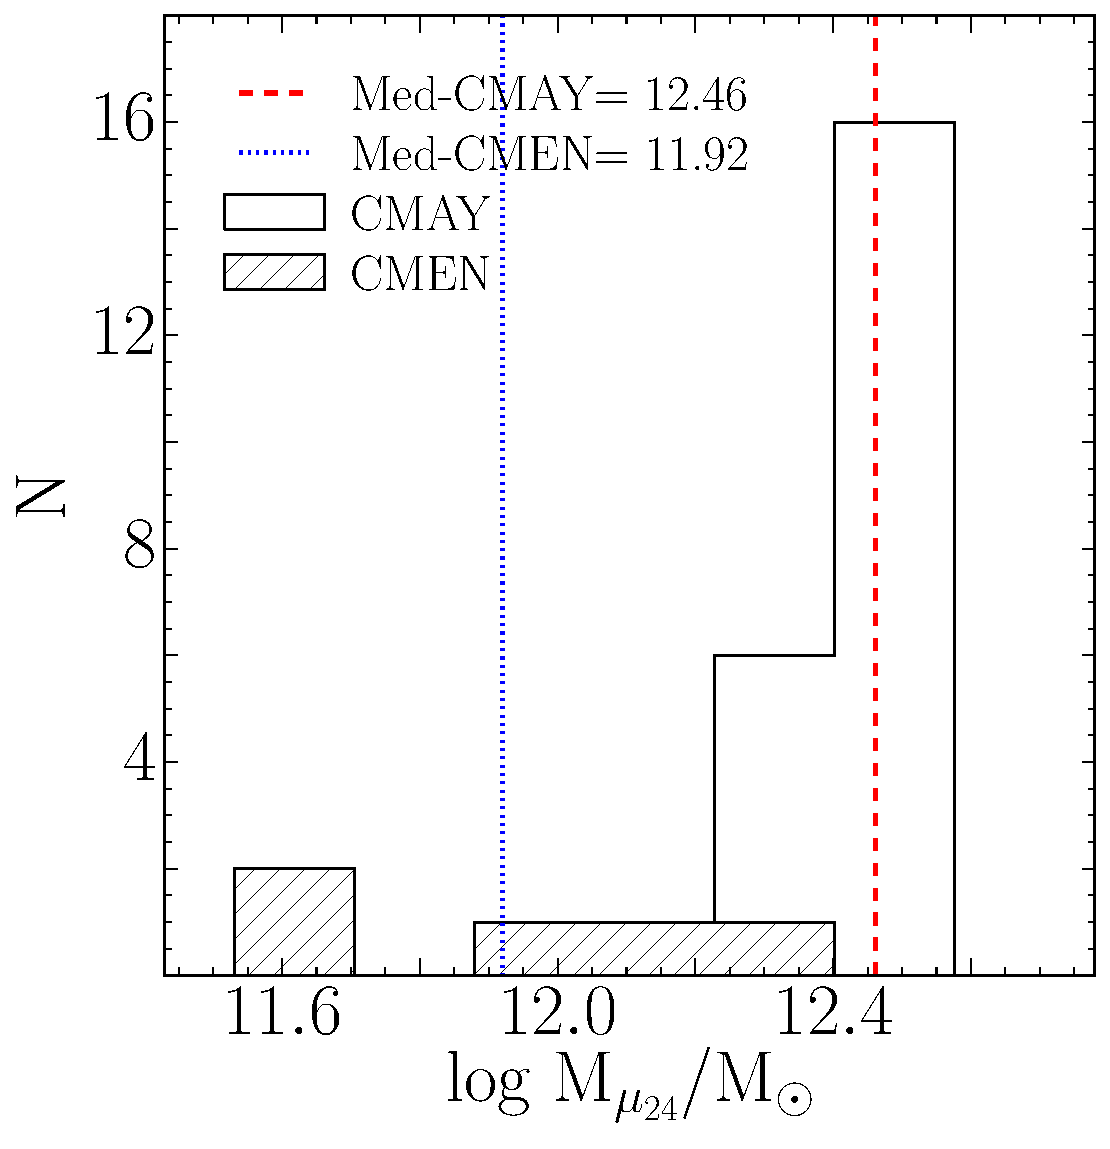
\includegraphics[height=9cm, width=9cm]{../al_final/LR/evolucion/histogramas/Mmu_grandes_chicasz0.pdf}
\end{figure}
\begin{figure}[H]
 \centering
 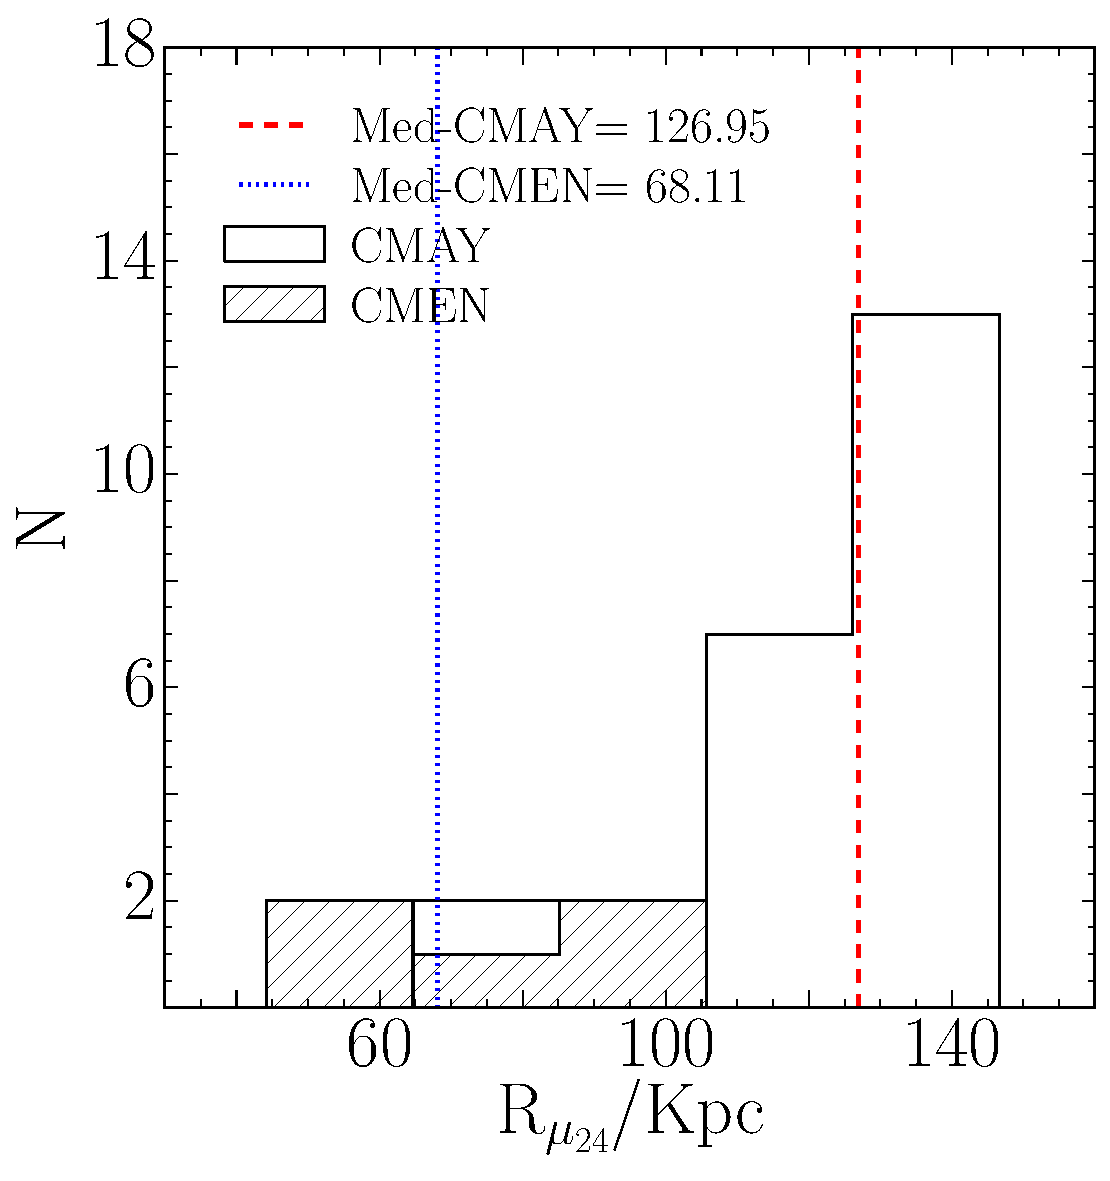
\includegraphics[height=9cm, width=9cm]{../al_final/LR/evolucion/histogramas/R24_grandes_chicasz0.pdf}
\end{figure}
\begin{figure}[H]
 \centering
 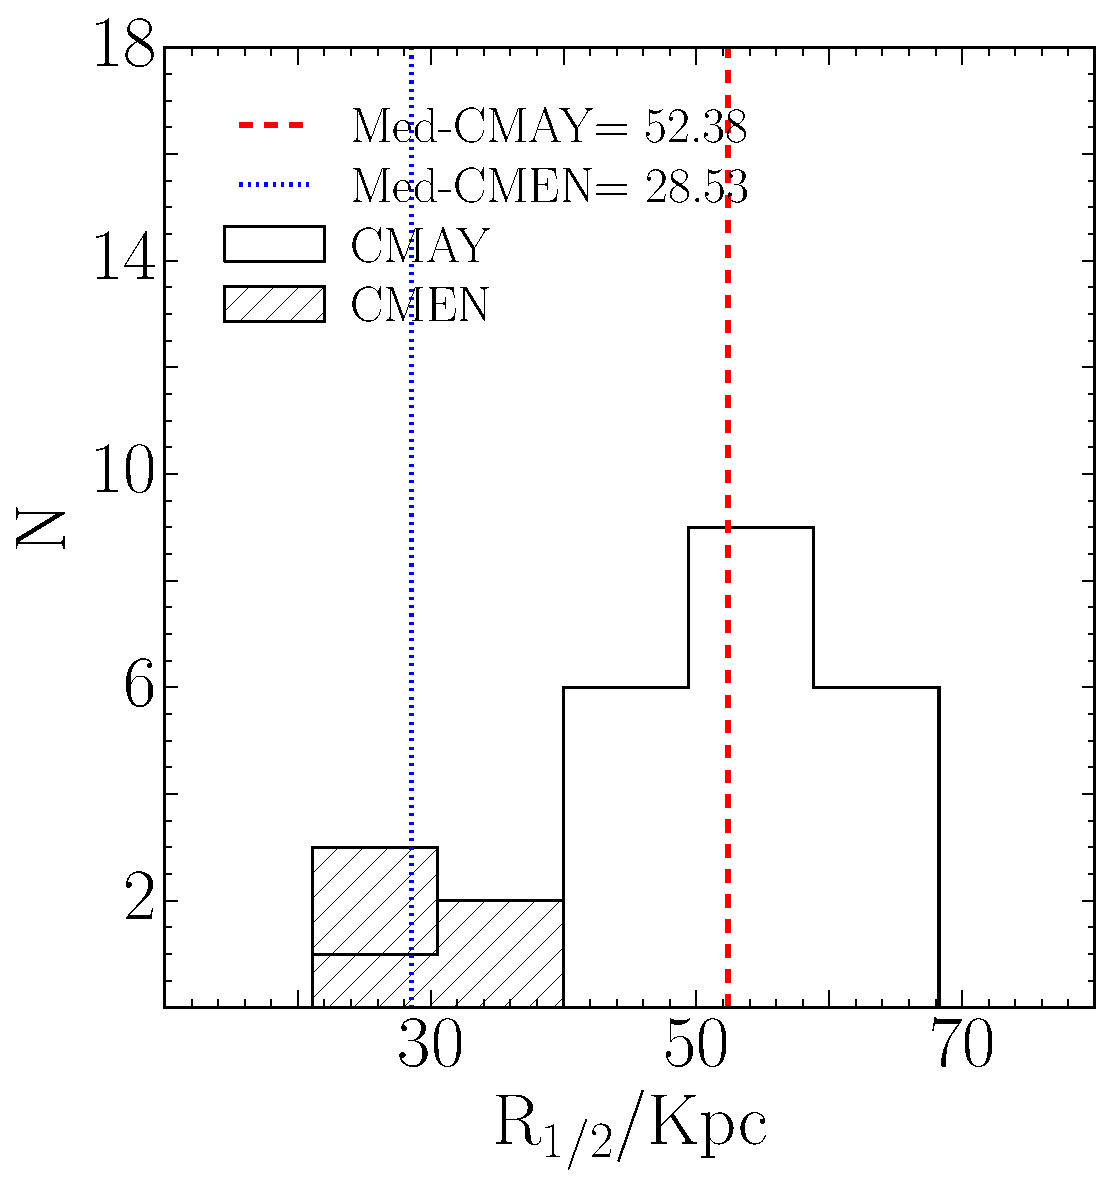
\includegraphics[height=9cm, width=9cm]{../al_final/LR/evolucion/histogramas/R50_grandes_chicasz0.pdf}
\end{figure}



\section{Relaciones Masa-Masa C\'umulo}

\begin{figure}[H]
 \centering
 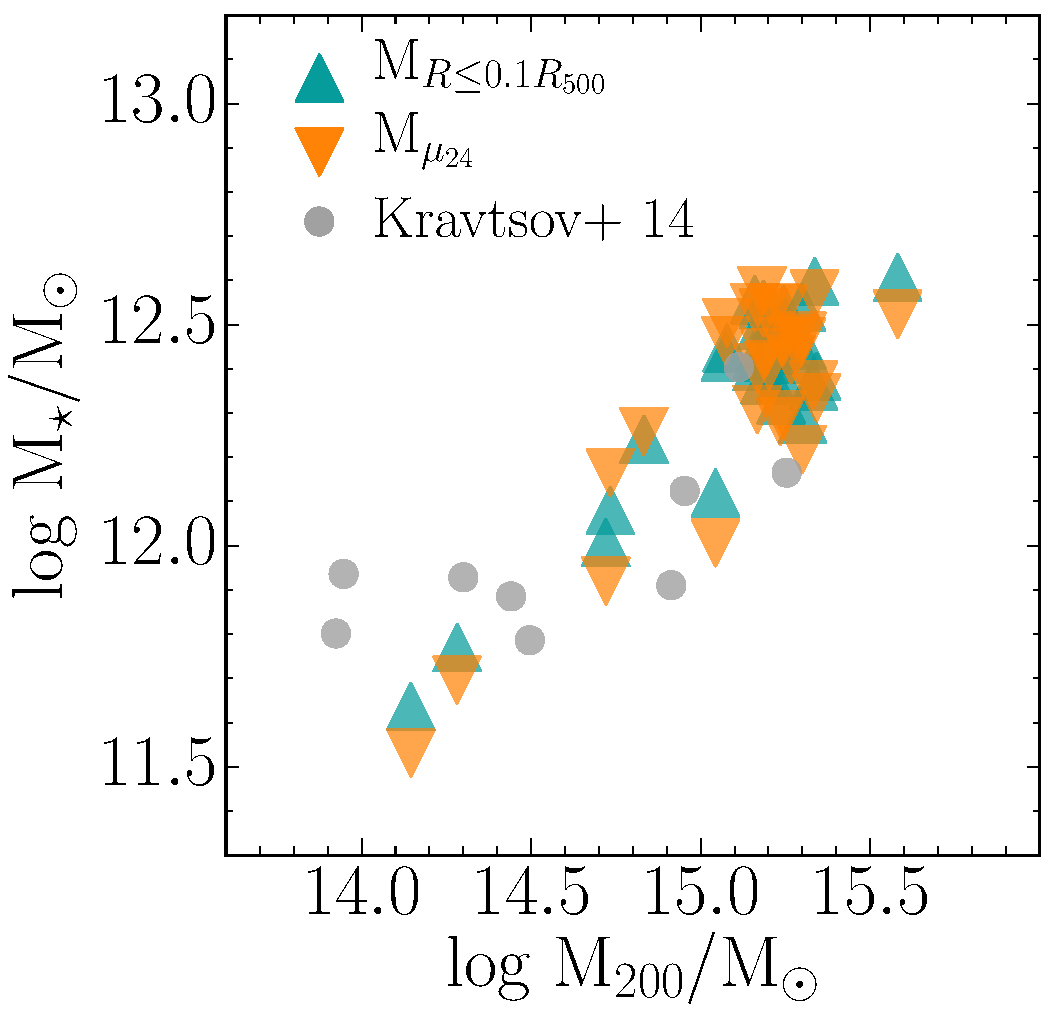
\includegraphics[height=9cm, width=10cm]{../al_final/LR/evolucion/relaciones/mtotales.pdf}
\end{figure}

\begin{figure}[H]
 \centering
 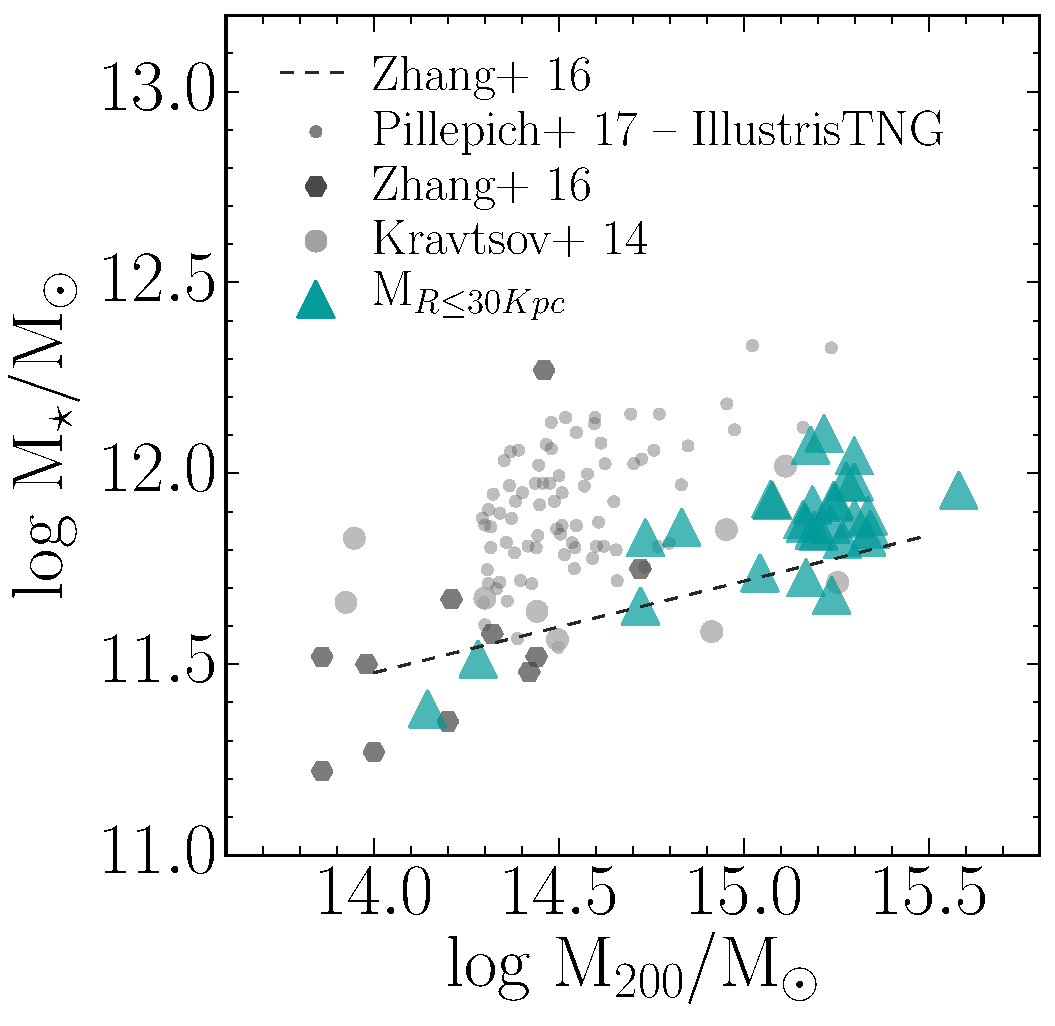
\includegraphics[height=9cm, width=10cm]{../al_final/LR/evolucion/relaciones/M302D_vs_M200.pdf}
\end{figure}

\begin{figure}[H]
 \centering
 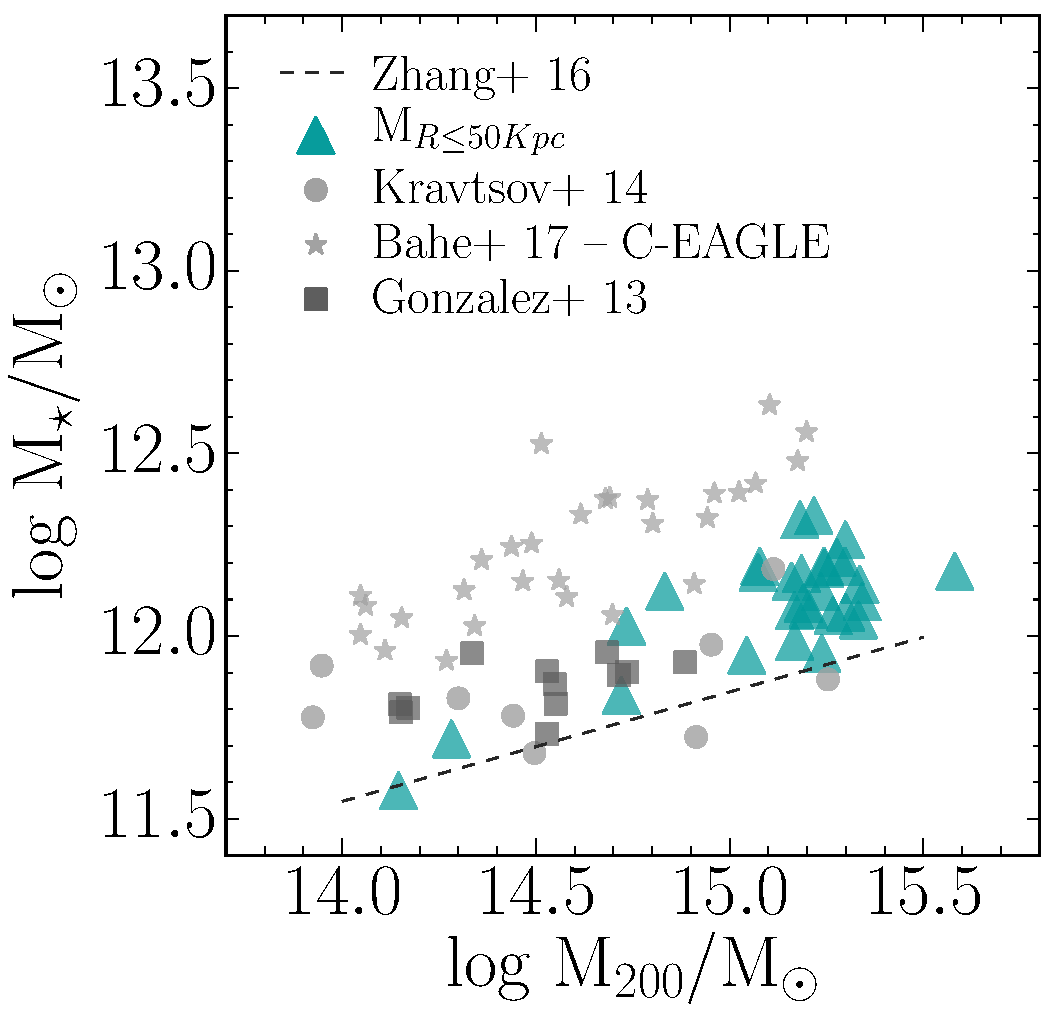
\includegraphics[height=9cm, width=10cm]{../al_final/LR/evolucion/relaciones/M502D_vs_M200.pdf}
\end{figure}



\section{Masas de las BCGs a distintos z}
\label{sec:zeta0}



\begin{figure}[H]
\centering
\hspace*{-1.5cm}
 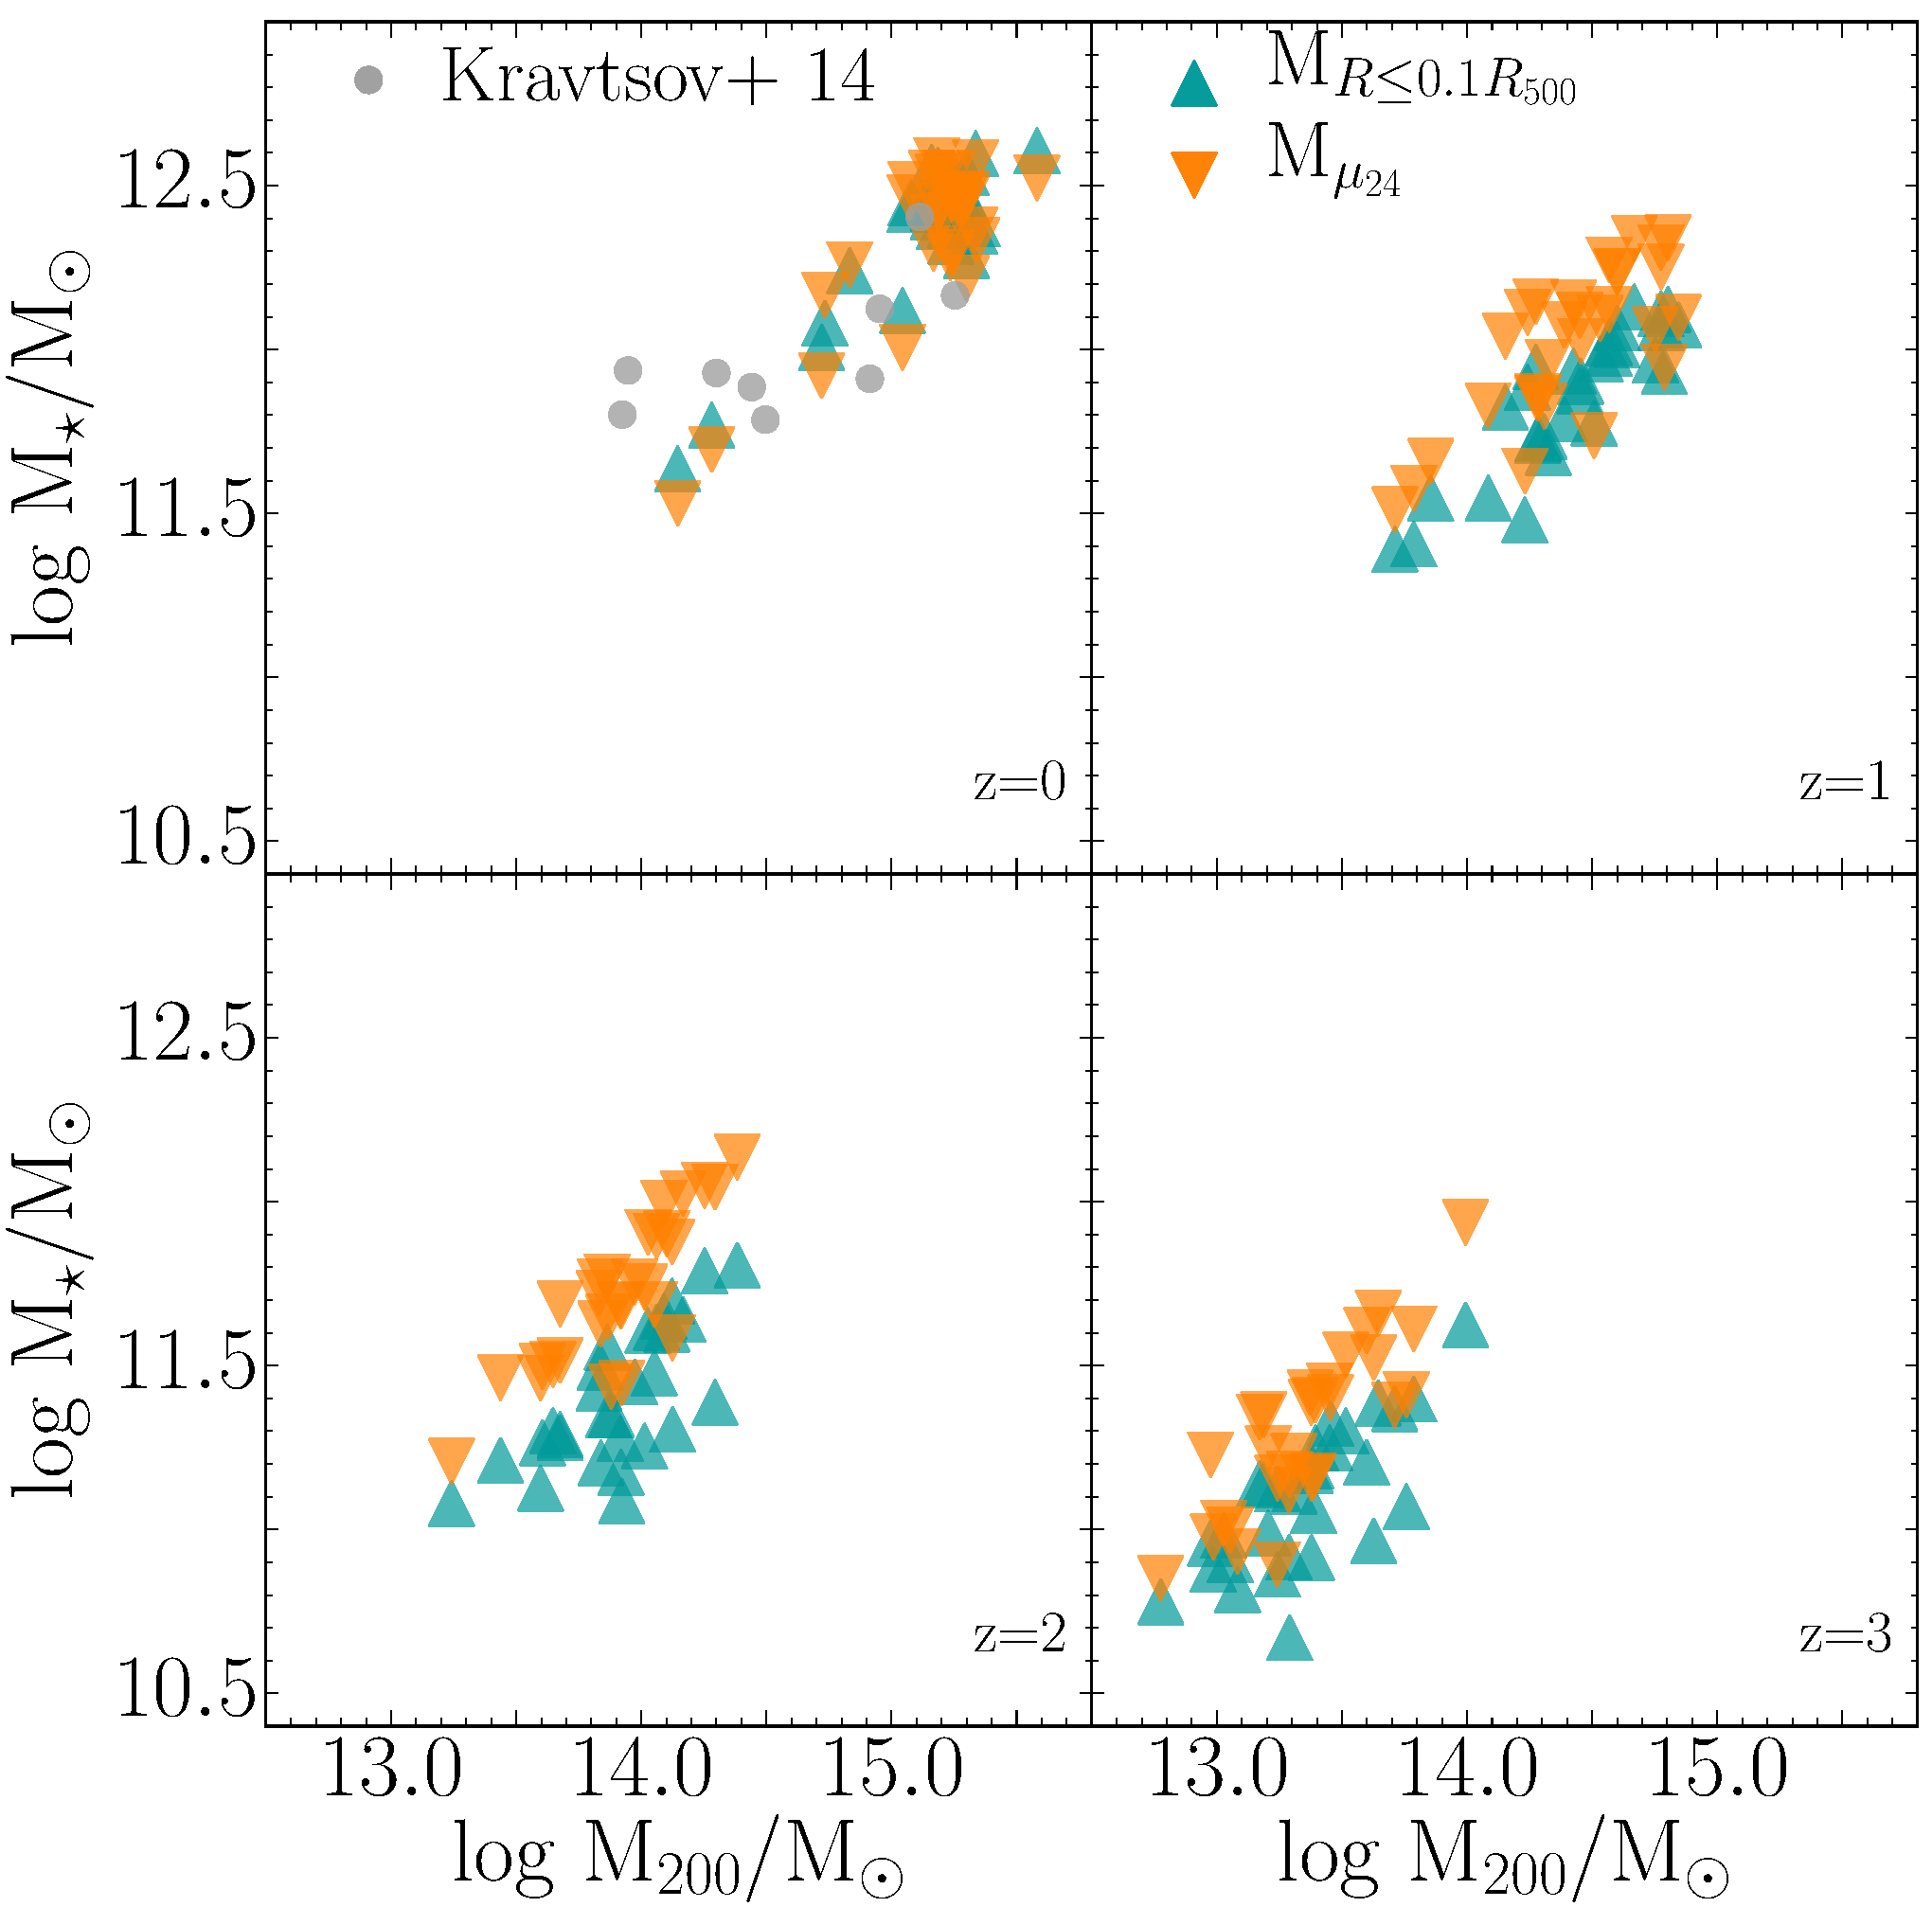
\includegraphics[height=12cm, width=13cm]{../al_final/LR/evolucion/relaciones/muvs10r.pdf}
\end{figure}

\begin{figure}[H]
\centering
\hspace*{-1cm}
 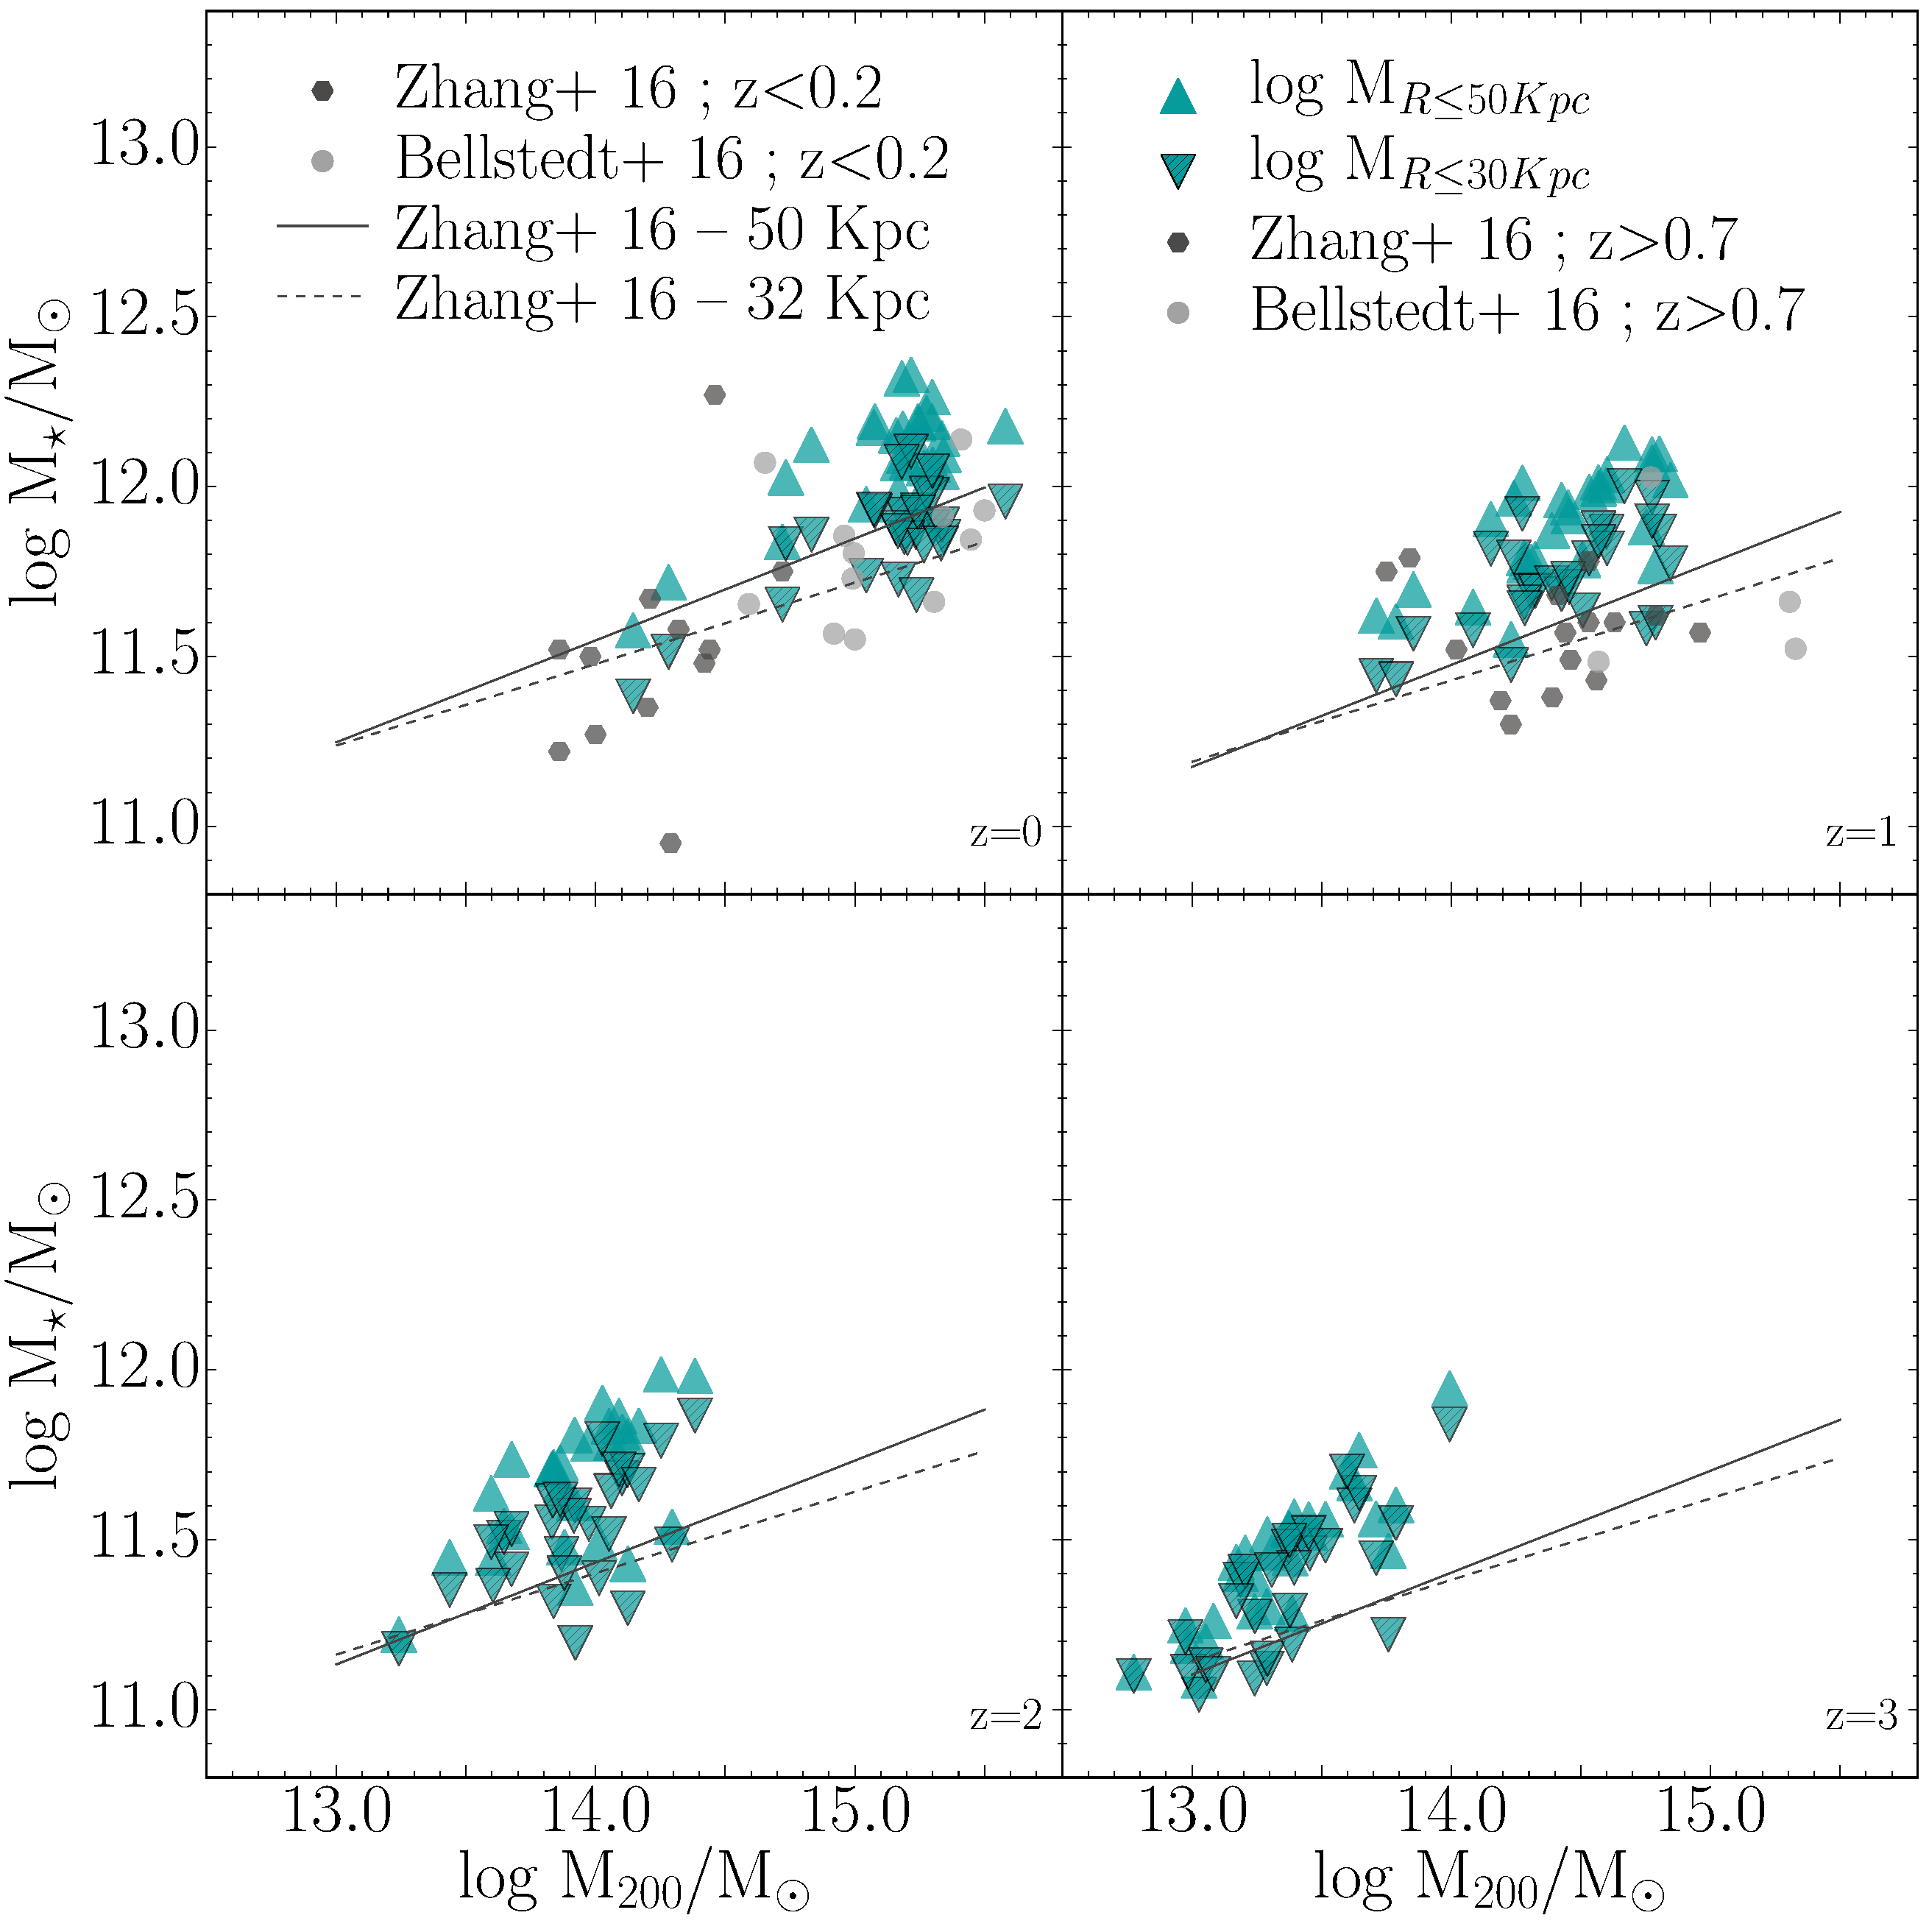
\includegraphics[height=12cm, width=13cm]{../al_final/LR/evolucion/relaciones/zhang_vs_z.pdf}
\end{figure}

ver: There is also a (weak) correlation between BCG mass and the mass of their host clusters, which does not change significantly
with redshift out to $z\sim 0.8 (Edge 1991; Collins & Mann 1998; Burke, Collins & Mann 2000; Brough et al. 2007; Stott et al. 2008;
Whiley et al. 2008).$

\section{evolucion en masa}

\begin{figure}[H]
 \centering
 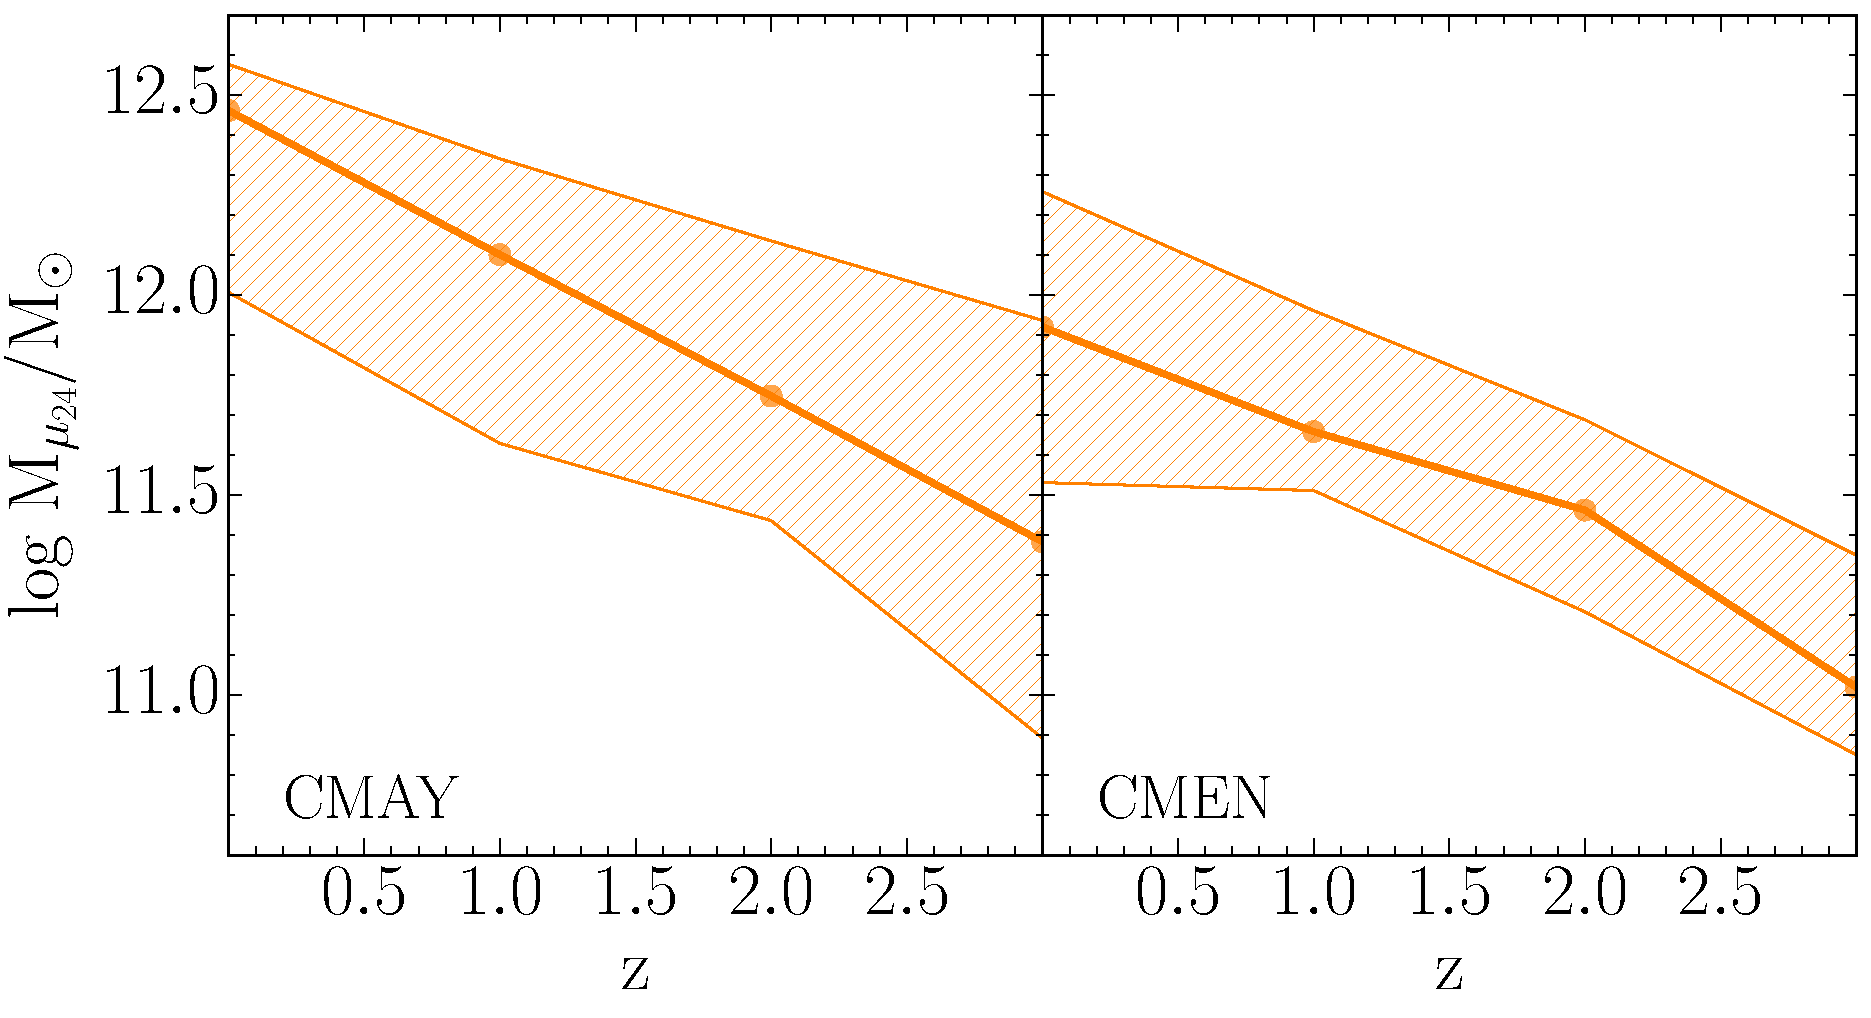
\includegraphics[height=7cm, width=14cm]{../al_final/LR/evolucion/observacional/evolucion_M24.pdf}
\end{figure}

\begin{figure}[H]
 \centering
 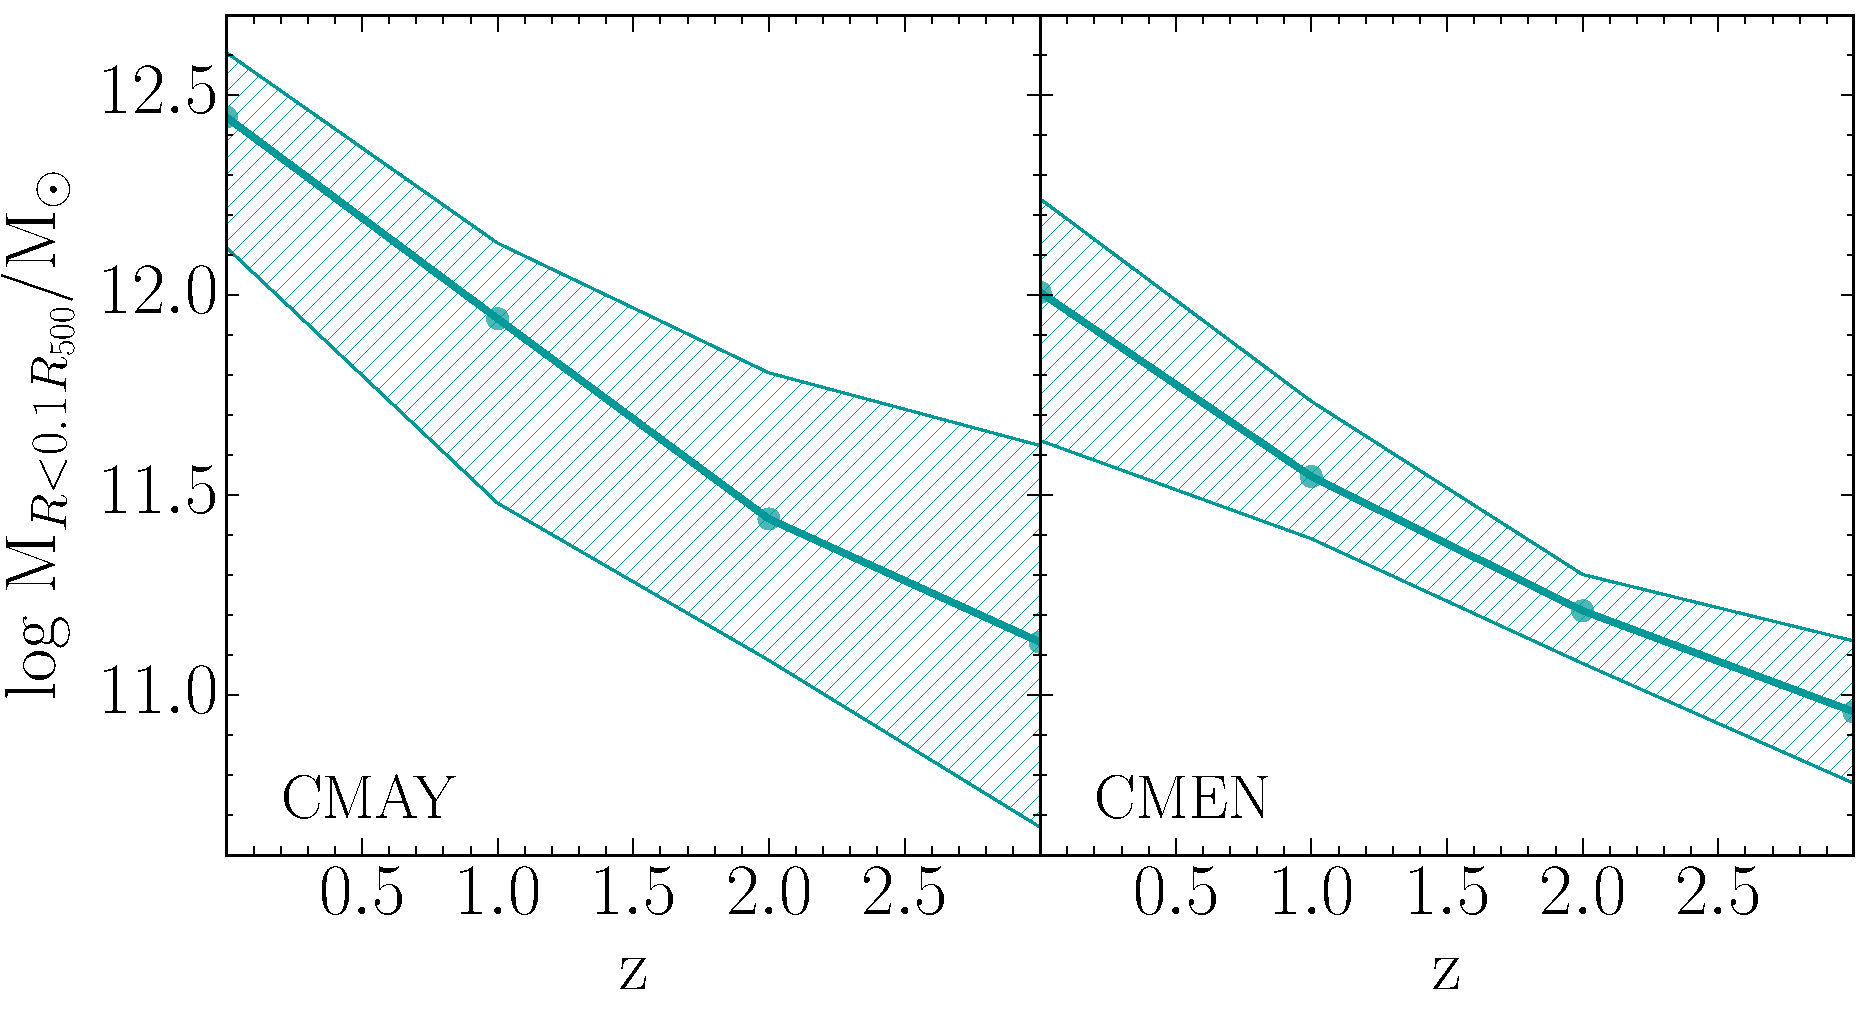
\includegraphics[height=7cm, width=14cm]{../al_final/LR/evolucion/simulacion/evolucion_M10_grandes_chicas.pdf}
\end{figure}


\begin{figure}[H]
 \centering
 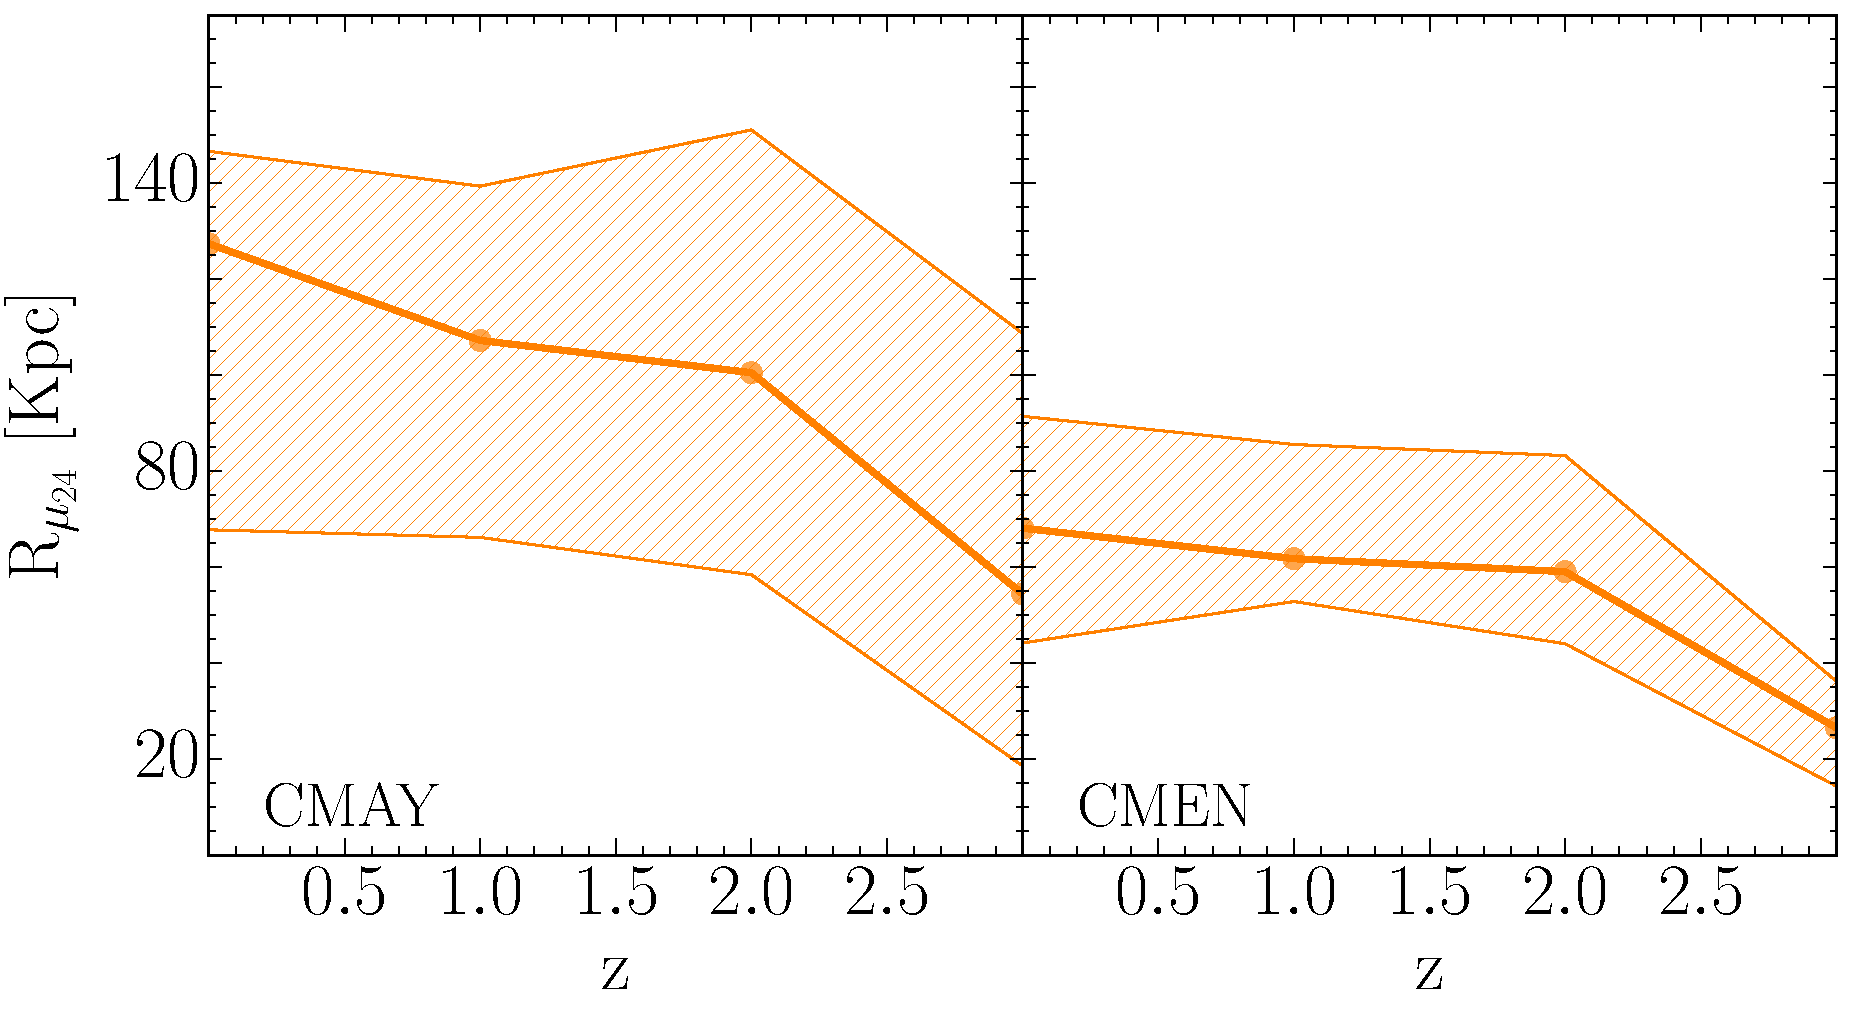
\includegraphics[height=7cm, width=14cm]{../al_final/LR/evolucion/observacional/evolucion_R24.pdf}
\end{figure}

\begin{figure}[H]
 \centering
 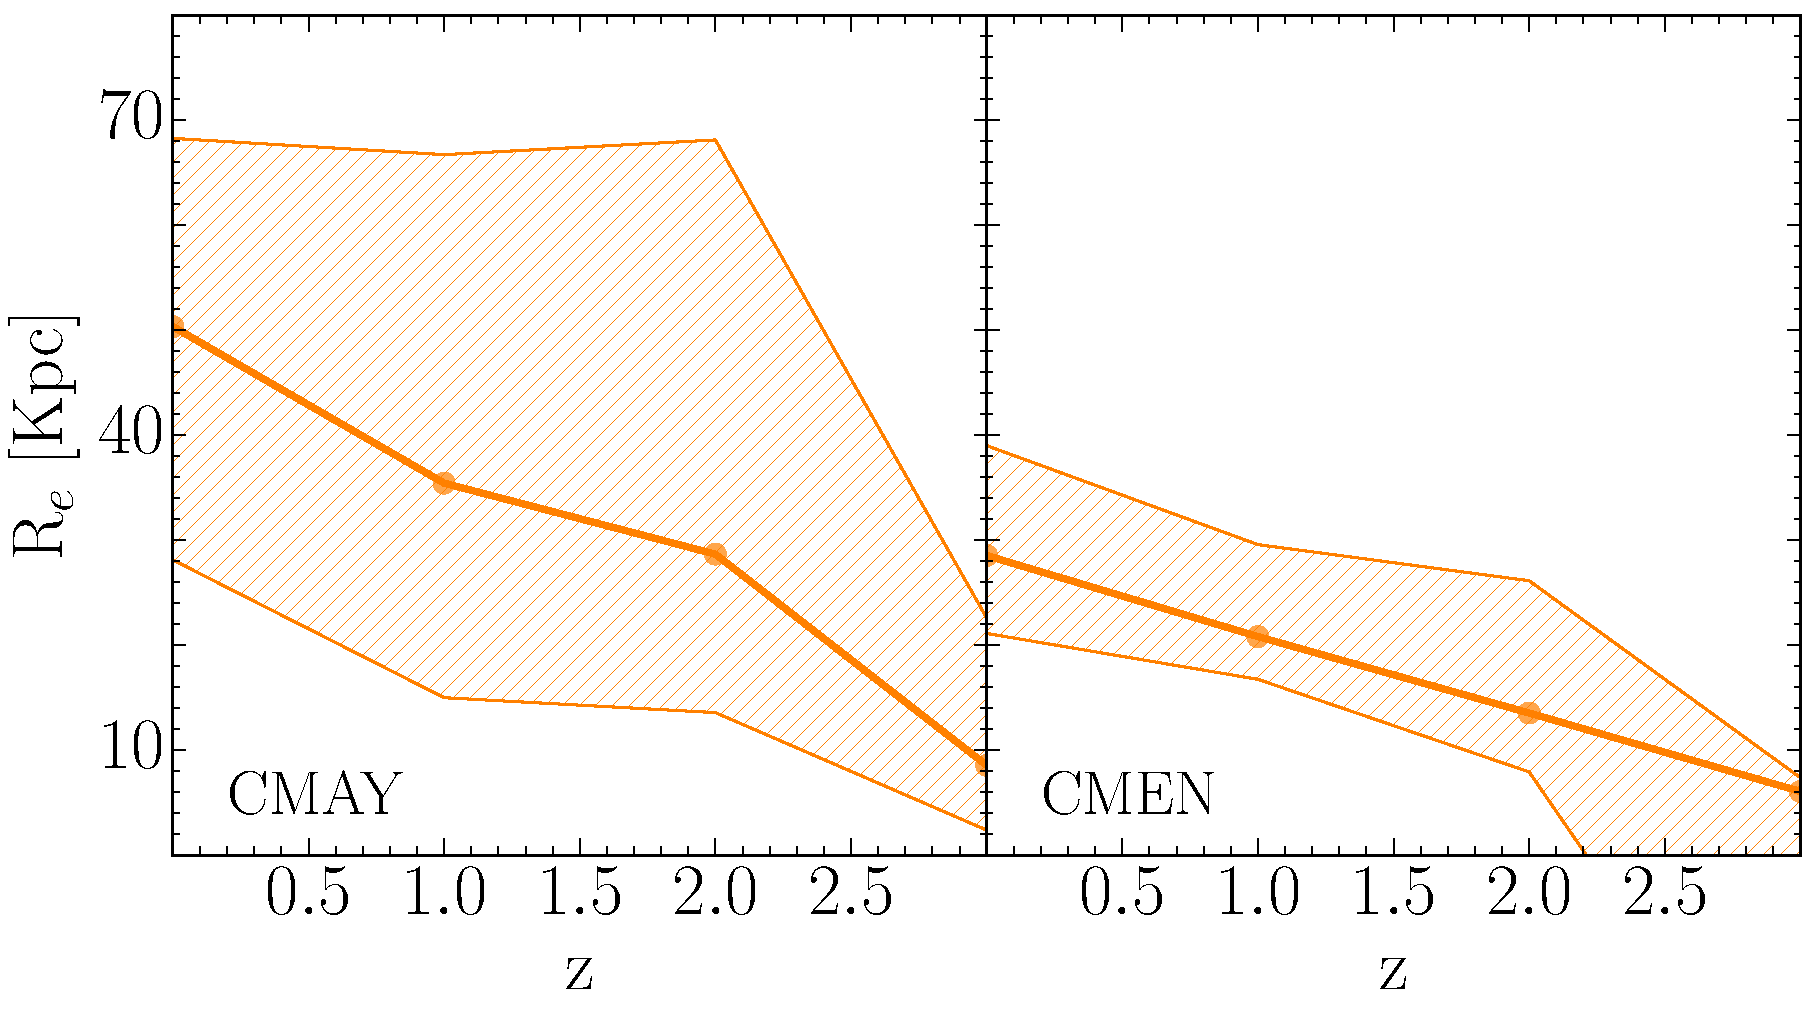
\includegraphics[height=7cm, width=14cm]{../al_final/LR/evolucion/observacional/evolucion_Re.pdf}
\end{figure}


\begin{figure}[H]
 \centering
 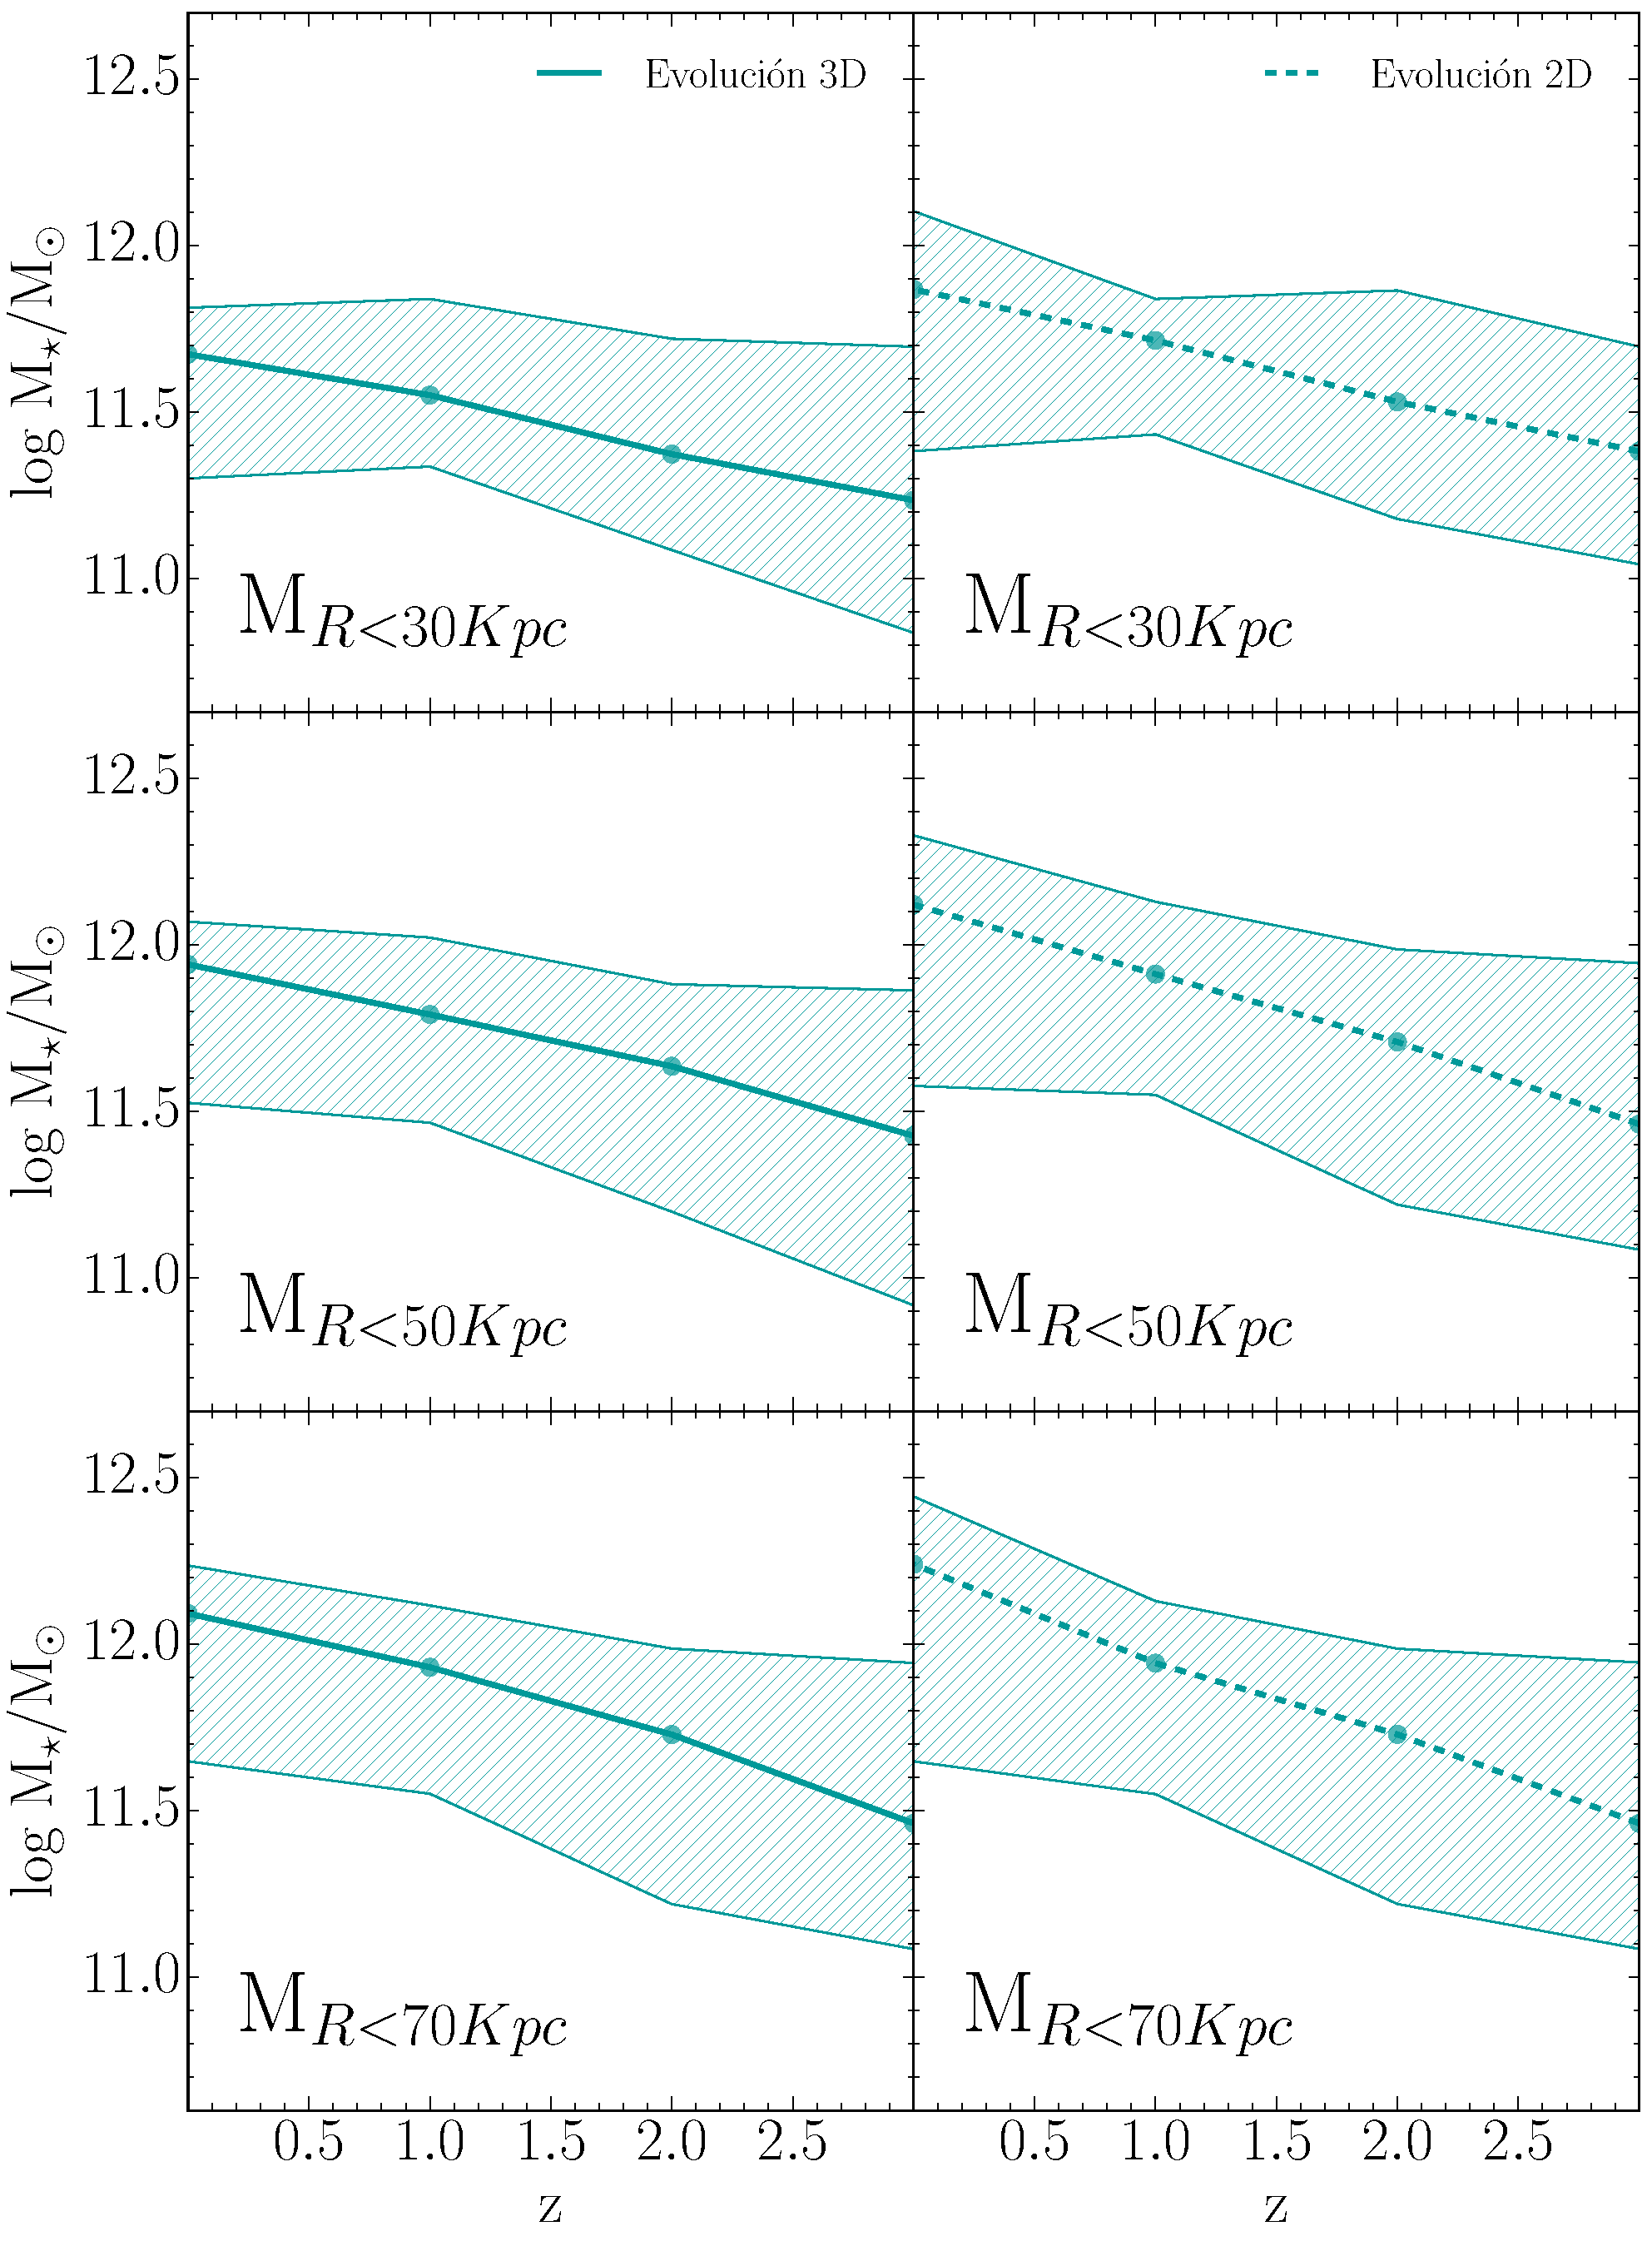
\includegraphics[height=18cm, width=14cm]{../al_final/LR/evolucion/simulacion/evolucion.pdf}
\end{figure}




\begin{figure}[H]
 \centering
 \includegraphics[height=7cm, width=7cm]{../al_final/LR/evolucion/histogramas/cocoientesmr24.pdf}
 \includegraphics[height=7.2cm, width=7cm]{../al_final/LR/evolucion/histogramas/cocoientesmr1medio.pdf}
 \\
 \includegraphics[height=7cm, width=7cm]{../al_final/LR/evolucion/histogramas/cocoientesm30r1medio}
 \includegraphics[height=7cm, width=7cm]{../al_final/LR/evolucion/histogramas/cocoientesm50r1medio}
\end{figure}


\section{evolucion en perfiles}

\begin{figure}[H]
 \includegraphics[height=24cm, width=15cm]{../al_final/plots/perfiles/bajustes_mues.pdf}
\end{figure}

\begin{figure}[H]
 \includegraphics[height=24.5cm, width=15cm]{../al_final/densidades/densidades.pdf}
\end{figure}



\section{edades y metalicidades}

\begin{figure}[H]
 \includegraphics[height=12cm, width=13cm]{../al_final/estrellas/stack/ultimoMETALICIDADES-PROG_zsunasplund.pdf}
\end{figure}

\begin{figure}[H]
 \includegraphics[height=12cm, width=13cm]{../al_final/estrellas/stack/ultimoEDADES-PROG_olivA.pdf}
\end{figure}


\begin{figure}[H]
 \includegraphics[height=7cm, width=7cm]{../al_final/estrellas/stack/ajustes/gradiente_edad_z0.pdf}
 \includegraphics[height=7cm, width=7cm]{../al_final/estrellas/stack/ajustes/gradiente_metalicidad_z0.pdf}
\end{figure}



\section{influencia del polvo. Solo a z=3 para algun dusty case}

\begin{figure}[H]
 \centering
 \includegraphics[height=7.5cm, width=7.5cm,trim={0cm   0.1cm 3.5cm 1.cm},clip ]{../al_final/LR/LR_minpot3_rmmax/nodust/grupo0/mu24/D1/026/maps_D1.pdf}
 \includegraphics[height=7.5cm, width=7.5cm,trim={2.8cm 0.1cm 0.3cm 1.cm},clip ]{../al_final/LR/LR_minpot3_rmmax/dust/grupo0/mu24/D1/026/maps_D1.pdf}
\end{figure}


\begin{figure}[H]
 \centering
 \includegraphics[height=7.5cm, width=7.5cm,trim={0cm   0.1cm 3.5cm 1.cm},clip ]{../al_final/LR/LR_minpot3_rmmax/nodust/grupo0/mu24/D22/026/maps_D22.pdf}
 \includegraphics[height=7.5cm, width=7.5cm,trim={2.8cm 0.1cm 0.3cm 1.cm},clip ]{../al_final/LR/LR_minpot3_rmmax/dust/grupo0/mu24/D22/026/maps_D22.pdf}
\end{figure}

\begin{figure}[H]
 \includegraphics[height=8.5cm, width=8.5cm,trim={0cm 0.1cm 0.cm 0.cm},clip]{../al_final/LR/LR_minpot3_rmmax/polvo_nopolvo1b3.pdf}
 \includegraphics[height=8.5cm, width=7.1cm,trim={2.9cm 0.1cm 0.2cm 0.cm},clip]{../al_final/LR/LR_minpot3_rmmax/polvo_nopolvo1D22.pdf}
\end{figure}


\begin{figure}[H]
\centering
 \includegraphics[height=8.5cm, width=8.5cm,trim={0cm 0.1cm 0.cm 0.cm},clip]{../al_final/plots/seds/plots_seds/sed_D1.pdf}
 %\includegraphics[height=8.5cm, width=7.1cm,trim={2.9cm 0.1cm 0.3cm 0.cm},clip]{../al_final/plots/seds/plots_seds/sed_D22.pdf}
\end{figure}


\begin{figure}[H]
 \centering
 \includegraphics[height=9cm, width=9cm]{../al_final/LR/evolucion/histogramas/Mmu_polvo_vs_nopolvo.pdf}
\end{figure}


\section{Estabilidad a High Resolution}
\begin{figure}[H]
 \centering
 \includegraphics[height=10cm, width=11cm]{../al_final/LR/evolucion/MRvsLR/mr_vs_lr.pdf}
\end{figure}

\begin{figure}[H]
 \hspace*{-1.4cm}\includegraphics[height=6.cm, width=6.3cm    ,trim={0cm   0.1cm 4.7cm 1.38cm},clip ]{../al_final/LR/LR_minpot3_rmmax/nodust/grupo0/mu24/D2/091/contoursmaps125.pdf}
  \hspace*{-.1cm}\includegraphics[height=6.cm, width=5.2cm,trim={2.5cm 0.1cm 4.7cm 1.38cm},clip ]{../al_final/MR/MR_minpot3_rmmax/nodust/grupo0/mu24/D2/091/contoursmaps125.pdf}
  \hspace*{-.1cm}\includegraphics[height=6.cm, width=6.9cm,trim={2.5cm 0.1cm 0.3cm 1.38cm},clip ]{../al_final/HR/HR_minpot3_rmmax/nodust/grupo0/mu24/D2/091/contoursmaps125.pdf}
\end{figure}


\begin{figure}[H]
  \hspace*{-1.4cm}\includegraphics[height=6cm, width=6cm,trim={0cm   0.cm 0.cm 0.cm},clip ]{../al_final/resoluciones/res1.pdf}
  \hspace*{.1cm}\includegraphics[height=6cm, width=5.4cm ,trim={2.3cm  0.cm 0.cm 0.cm},clip ]{../al_final/resoluciones/res2.pdf}
  \hspace*{.1cm}\includegraphics[height=6cm, width=5.4cm ,trim={2.3cm  0.cm 0.cm 0.cm},clip ]{../al_final/resoluciones/res3.pdf}
\end{figure}

\section{Relaciones de Escala}



\begin{figure}[H]
 \centering
 \includegraphics[height=9.5cm, width=10cm]{../al_final/plots/parametros_de_escala/mevsm_medians.pdf}
\end{figure}

\begin{figure}[H]
 \centering
 \includegraphics[height=9.5cm, width=10cm]{../al_final/plots/parametros_de_escala/nvsm_medians.pdf}
\end{figure}

\begin{figure}[H]
 \centering
 \includegraphics[height=9.5cm, width=10cm]{../al_final/plots/parametros_de_escala/revsm_medians.pdf}
\end{figure}

\begin{figure}[H]
 \centering
 \includegraphics[height=10cm, width=11cm]{../al_final/plots/parametros_de_escala/kormendy.pdf}
\end{figure}
 
\chapter{Conclusiones} 

%----------------------------------------------------------------------------------------
%	THESIS CONTENT - APPENDICES
%----------------------------------------------------------------------------------------

\appendix % Cue to tell LaTeX that the following "chapters" are Appendices

% Include the appendices of the thesis as separate files from the Appendices folder
% Uncomment the lines as you write the Appendices

% Appendix A

\chapter{Frequently Asked Questions} % Main appendix title

\label{AppendixA} % For referencing this appendix elsewhere, use \ref{AppendixA}

\section{How do I change the colors of links?}

The color of links can be changed to your liking using:

{\small\verb!\hypersetup{urlcolor=red}!}, or

{\small\verb!\hypersetup{citecolor=green}!}, or

{\small\verb!\hypersetup{allcolor=blue}!}.

\noindent If you want to completely hide the links, you can use:

{\small\verb!\hypersetup{allcolors=.}!}, or even better: 

{\small\verb!\hypersetup{hidelinks}!}.

\noindent If you want to have obvious links in the PDF but not the printed text, use:

{\small\verb!\hypersetup{colorlinks=false}!}.

%\include{Appendices/AppendixB}
%\include{Appendices/AppendixC}

%----------------------------------------------------------------------------------------
%	BIBLIOGRAPHY
%----------------------------------------------------------------------------------------

\printbibliography[heading=bibintoc]

%----------------------------------------------------------------------------------------

\end{document}  
